\documentclass{kththesis}

\usepackage{csquotes} % Recommended by biblatex
\usepackage[style=numeric,sorting=none,backend=biber]{biblatex}
\addbibresource{references.bib} % The file containing our references, in BibTeX format
%\usepackage[T1]{fontenc} needed for black boxes in bibliography?


\usepackage{amsmath,amsthm, amssymb}
\usepackage[ruled,vlined,linesnumbered]{algorithm2e}  % for BO-DMIX algo
\usepackage{wrapfig}
\usepackage{amsfonts}
\usepackage{booktabs}
% \usepackage{float}
\usepackage{subcaption}
\usepackage{rotating}
\usepackage{overpic}
\usepackage[outercaption]{sidecap}  


\usepackage{nameref}
% For \ang
\usepackage{siunitx}

\usepackage[font={small}]{caption} % To make image captions smaller
\usepackage[colorinlistoftodos]{todonotes}
\usepackage{mathtools}
% \usepackage{color}
%\usepackage{hyperref}
%\usepackage{verbatim}
\usepackage{tikz}
\usetikzlibrary{arrows.meta,positioning,bayesnet,backgrounds,calc,decorations.pathreplacing}
\usepackage{enumitem}  % for tighter list spacing
\usepackage{hyperref} % for URLs

% Smaller bullets in lists.
\newlength{\mylen}
% \setbox1=\hbox{$\bullet$}\setbox2=\hbox{\tiny$\bullet$}
% \setlength{\mylen}{\dimexpr0.5\ht1-0.5\ht2} 
% \setlist[itemize]{itemsep=0mm, topsep=2pt}

%======================================================
\newcommand{\vz}{\boldsymbol{z}}
\newcommand{\vx}{\boldsymbol{x}}
\newcommand{\vy}{\boldsymbol{y}}
\newcommand{\vth}{\boldsymbol{\theta}}
\newcommand{\vph}{\boldsymbol{\phi}}
\newcommand{\vpsi}{\vec{\psi}}

\DeclareMathOperator{\E}{\mathbb{E}}
\renewcommand{\vec}[1]{\boldsymbol{#1}}

\makeatletter
\newcommand{\@givennoparenthesis}[2]{\ensuremath{{{#1}\;\middle|\;{#2}}}}
\newcommand{\givennop}{\@givennoparenthesis}
\newcommand{\@giventhatstar}[2]{\ensuremath{\left({#1}\;\middle|\;{#2}\right)}}
\newcommand{\@giventhatnostar}[3][]{#1(#2\,#1|\,#3#1)} 
\newcommand{\given}{\@ifstar\@giventhatstar\@giventhatnostar}
\makeatother
 
\DeclarePairedDelimiterX{\infdivx}[2]{\big(}{\big)}{%
  #1\;\delimsize\|\;#2%
}
\newcommand{\KL}{D_{\mathcal{KL}}\infdivx}
\newcommand{\N}{\mathcal{N}}

\newcommand{\vae}{\textsc{vae}}
\newcommand{\cvae}{\textsc{cvae}}
\newcommand{\dettostoc}{\textsc{det2stoc}}

\newcommand{\vs}{\pmb{s}_t}
\newcommand{\va}{\pmb{a}_t}
\newcommand{\vns}{\pmb{s}_{t+1}}

\newcommand{\fsimulator}{\ensuremath{f^{sim}}}
\newcommand{\fpsisimulator}{\ensuremath{f^{sim}_{\psi}}}
\newcommand{\fdecoder}{\ensuremath{f^{decoder}}}
\newcommand{\fencoder}{\ensuremath{f^{encoder}}}
% \newcommand{\fdecoder}{\ensuremath{f_{\phi_{decoder}}}}

\newcommand{\ra}[1]{\renewcommand{\arraystretch}{#1}}

\newcommand{\pfriction}{\psi_{\textsc{friction}}}
\newcommand{\pcom}{\psi_{\textsc{com}}}
\newcommand{\pwind}{\psi_{\textsc{wind}}}

\newcommand{\ptheta}{p_{\theta}}
\newcommand{\qphi}{q_{\phi}}

\newcommand{\trajsim}{\xi^{sim}}
\newcommand{\trajreal}{\xi^{real}}

\newcommand{\ws}{Windy Slope}
\newcommand{\yp}{YuMi Pusher}

% Used when drawing neural nets
\def\nodesize{30pt}
\def\smallnodesize{20pt}
\def\nodesep{12pt}
\def\smallnodesep{6pt}
\def\layersep{16pt}
\definecolor{rose}{HTML}{ffa9b5}
\definecolor{curry}{HTML}{f6c800}
\definecolor{moss}{HTML}{757b33}

%======================================================

\title{det2stoc -- Converting Deterministic Simulators to Realistic Stochastic Models via Data Alignment}
\alttitle{det2stoc -- Omvandla Deterministiska Simulatorer till Realistiska Stokastiska Modeller via Data Justering.}
\author{Martin Hwasser}
\email{hwasser@kth.se}
\supervisor{Rika Antonova}
\examiner{Danica Kragic}
\programme{Master in Computer Science}
\school{School of Electrical Engineering and Computer Science}
\date{\today}

\kthcover{kth-cover.pdf}

\begin{document}
\frontmatter
\titlepage
% ======================================================
% ABSTRACT
% ======================================================
\begin{abstract}
Simulation is commonly used to train agents in Reinforcement Learning since they provide an affluence of data that in many cases can be generated faster than real-time. However, the behaviors learned by the agent will be specific to attributes of the simulator and may not perform well when transfered to the real world. This thesis describes an algorithm that can be used to minimize the discrepancy between simulation and reality. Using this algorithm, it is possible to both identify parameters of the simulator whose true values are unknown, as well as replacing a deterministic simulator with a generative model that can produce output that is close to real-world dynamics.

We first demonstrate this algorithm on a problem that can be solved analytically. We then show that the algorithm can be applied to more elaborate environments with physics simulation involving contact between objects and control actions.

%And finally, we show that the algorithm can be used to facilitate training an agent in simulation and transferring the learned policy to a real robot.
\end{abstract}
\begin{otherlanguage}{swedish}
  \begin{abstract}
    \todo[inline]{En abstract på svenska.}
  \end{abstract}
\end{otherlanguage}

\section*{Acknowledgements}

This thesis would not have been possible without my supervisor Rika Antonova, whose expertise paved the way for the methodology in this work. Ever the inspiring mentor; demanding more when I made progress and being patient when I struggled, whether in regard to the thesis or hardships in my personal life. Always available for a discussion, and unfailingly replying within an instant to emails in the middle of the night.Thank you.

% ======================================================
\tableofcontents
% ======================================================
\mainmatter
% ======================================================

\chapter{Introduction}
\label{introduction}
For many applications in Machine Learning (ML), and in particular for learning complex continuous control, training is often performed in simulation rather than in the real world. Data is abundant in simulation and can often be generated faster than real-time, being limited strictly by computing power. In contrast, collecting data in the real world is arduous, expensive and time consuming. When training agents using Reinforcement Learning (RL), the training process might also cause safety concerns. Since a key component of learning is exploration, it is possible that an agent executes actions that pose a danger to itself or its environment.

However, simulation comes with drawbacks: a model trained solely in simulation may behave very differently when transferred to the real world due to modelling errors, insufficiently accurate physics engines and lack of high fidelity simulation environments. Furthermore, while simulation can provide useful initial indicators for the potential of various RL algorithms, it cannot reliably predict RL performance for real robotics systems. Many RL tasks depend heavily on the physical properties of the system, and although sophisticated simulation engines offer a wide range of adjustable parameters, it is neither guaranteed that correct values correspond to the most accurate simulation of reality, nor can each and every parameter accurately be measured in isolation. An important research area is thus minimizing the discrepancy, or \emph{reality gap} \parencite{Jakobi1995NoiseAT}, between simulation and reality, resulting in more robust behavior and reducing time spent training in the real world. This research field is also known as Simulation-to-Real (Sim-to-Real).

\section{Research Question}

Consider a general-purpose simulator. Using known physics laws, it can be viewed as defining a deterministic function $f_{\vph}(\vs, \va) \rightarrow \vns$ that returns the next state $\vns$ given current state $\vs$ and control actions $\va$ at time $t$. This function is ''parameterized'' by our choice of variables $\vph$ that describe the environment (such as inertial and frictional properties of robot and objects) as well as configurations of the simulator software (e.g. choice of integrator, choice of parameters that influence how contacts are computed). Simulators describe well the general behavior of the system, but contain parameters that are infeasible to estimate precisely.%, such as damping properties of the joints.

Given a sufficiently precise and flexible simulator, the parameters $\vph$ could be tuned such that $f_{\vph}(\vs, \va) \rightarrow \vns$ matches the mean of the real world behavior. However, it is not realistic to expect to find the exact deterministic function and parameters $\vph$ that specify dynamics of interactions in the real world.

A deterministic solution is generally not desirable, and instead, to capture the uncertainty of real-world data, we wish to model a stochastic distribution. A state-of-the-art solution is learning a probabilistic function $g(\cdot)$, such that the stochastic part of the function yields a probability distribution over next states $\vns$ given states $\vs$ and actions $\va$.

Building a generative model ''from scratch’' using real world data is not data-efficient. Instead, we propose to learn the parameters $\vph$ by aligning the output of an existing physics simulator with a small set of real-world observations. In this work, we investigate a data-driven approach that explores how real observations can be combined with general-purpose simulators to make learning of the stochastic function $g(\cdot)$ more data efficient.

\section{Contributions}

The main contribution of this thesis is the algorithm \dettostoc{}, a data-efficient solution to learn a generative model by aligning a physics simulator with real-world observations.

\section{Ethics, societal aspects and sustainability}

As a research topic, Sim-to-Real has major impact on the world. With current learning techniques it is not feasible to learn complex RL tasks with few samples. This means simulation is of tremendous significance in the development of machine intelligence. Enabling intelligent systems and robots to interact with their environment at the skill level of humans will have substantial impact on society. The future may be vast of robots performing everything from mundane, everyday chores to complex tasks that are hazardous to humans. As with any technical revolution, the living standard for some people will increase, while other people will inevitably lose their job. As such, there needs to be a system in place to support affected people when it happens and assist and rehabilitate transition into other professions or reeducation. This redistribution of needs and labour can in turn have an effect on the economy. We can also not ignore the importance of robots in controversial and potentially malicious practices such as armed drones.

%As the focus on this thesis is ultimately to simulate reality better, it can be utilized in a variety of different research areas. Intelligent systems can have great beneficial impact on the world, from mundane chores such as vacuuming homes to tasks that are hazardous for humans. 

In essence, the effects of improving simulation has in itself no ethical impact but could enable or facilitate the learning of intelligent systems which comes with both positive and negative consequences.

\section{Overview of thesis}
The theoretical concepts behind deep learning and variational methods used in the project are presented in Chapter \ref{background}. This chapter also reviews the body of work done in the domains of dynamics randomization and Sim-to-Real transfer. Chapter \ref{methods} introduces the method, describes the \dettostoc{} algorithm and lists tools and motivation for the models used. The baseline architecture and proposed extensions are also presented in detail. Chapter \ref{experiments} describes the conducted experiments and obtained results. Chapter \ref{conclusions} summarizes the project work, draws conclusions, discusses encountered problems, and suggests potential future directions for the work.


\chapter{Background}
\label{background}
This chapter introduces the relevant theory required to follow the main aspects of the thesis. A deep conditional variational autoencoder (\cvae{}) was chosen to model the stochastic simulator. With that in mind, we start with a short introduction to deep learning and neural networks, and then move on to variational autoencoders (\vae{}) and variational inference. In the last part of the chapter we describe related work, specifically within the domains of transfer learning and Sim-to-Real.

%A \emph{variational autoencoder} (\vae{}) was chosen to model a stochastic simulator. A \vae{} is a probabilistic model, but relatively similar in spirit to standard non-probabilistic autoencoder. Both the autoencoder and the \vae{} employ neural networks and with that in mind, a short introduction to deep learning will be given in this chapter before more detailed description of \vae{} on which the methodology for this project builds upon.

\section{Deep neural networks}
\subsection{Neural networks}
The most basic form of neural network is a feedforward network, also known as a \emph{multilayer perceptron} (MLP). Feedforward networks constitute the foundation of deep learning and are in essence differentiable function approximators. That is, they approximate the function $\vy=f^{*}(\vx)$ using the mapping $\vy = f(\vx; \vth)$ and learn the parameters $\pmb{\theta}$ that best produce the desired output $\vy$.

A feedforward network takes the form of a \textit{computational graph}. A computational graph is a directed graph where each node is either a variable, such as input, or an operation. These operations are called \emph{hidden units} or \emph{neurons}, and are organized in groups called \emph{layers}. The graph describes how the input flows through these layers.
The feedforward network has a simple acyclic topology, or architecture, where all the nodes in one layer are connected to all the nodes in the next layer. An example can be seen in figure \ref{fig:mlp}.

The edges in the graph correspond to weights and are learnable parameters $\vth$ of the network. As such, a feedforward network is simply a composite function parameterized by the weights of the graph that maps some set of input values to some corresponding set of output values, through layers of functions stacked on top of each other in a chain. For example, a feedforward network with two hidden layers $h^{(1)}$, $h^{(2)}$ as in figure \ref{fig:mlp} would form the function composition $f(\vx) = h^{(2)}\big(h^{(1)}(\vx)\big)$.

Each hidden layer typically computes some affine transformation followed by a nonlinear transformation called \textit{activation function}. The nonlinearity of the activation functions is important as it increase the modeling capabilities of the network. Thus, adding more layers yields deeper and subsequently more powerful models, giving rise to the name \emph{deep} learning.
%\begin{equation}
%    a_j = \sum^D_{i=1} w^{(k)}_{j,i} x_i + b^{(k)}, \forall j=1\dotscM, \forall k=1 \dotsc K
%\end{equation}

%For some task, we want to predict the output $\boldsymbol{y}$ given some input $\vx$ and parameters $\boldsymbol{\theta}$. 

\begin{figure}
\captionsetup{width=\linewidth}
\centering
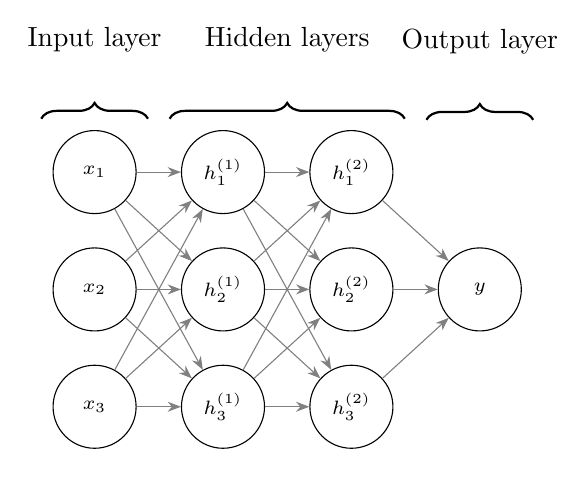
\begin{tikzpicture}[shorten >=0pt,->,draw=black!50,
    node distance=\nodesep and \layersep,
    myarrow/.style={-Stealth},
    brc/.style = {decorate, decoration={brace,amplitude=2mm},-,thick,black},inner sep=0pt]
    \scriptsize
    \tikzstyle{neuron}=[circle,draw=black,fill=white!50,minimum size=\nodesize,inner sep=0pt]
    \tikzstyle{input neuron}=[neuron];
    \tikzstyle{output neuron}=[neuron];
    \tikzstyle{hidden neuron}=[neuron];
    \tikzstyle{annot}=[text width=3em, text centered]

    % Draw the input layer nodes
    \node[input neuron] (I-1) at (0,0) {$x_1$};
    \foreach \name [count=\i] in {2,...,3}
        \node[input neuron, below=of I-\i] (I-\name) {$x_{\name}$};

    % Draw the hidden layer nodes
    \foreach \name in {1,...,3}
        \node[hidden neuron, right=of I-\name] (H1-\name) {$h^{(1)}_{\name}$};
        
    % Draw the hidden layer nodes
    \foreach \name in {1,...,3}
        \node[hidden neuron, right=of H1-\name] (H2-\name) {$h^{(2)}_{\name}$};

    % Draw the output layer node
    \node[output neuron, right=of H2-2] (O) {$y$};

    % Connect every node in the input layer with every node in the
    % hidden layer.
    \foreach \source in {1,...,3}
        \foreach \dest in {1,...,3}
            \draw [myarrow] (I-\source) -- node[sloped] {} (H1-\dest);
            
    \foreach \source in {1,...,3}
        \foreach \dest in {1,...,3}
            \draw [myarrow] (H1-\source) -- node[sloped] {} (H2-\dest);

    % Connect every node in the hidden layer with the output layer
    \foreach \source in {1,...,3}
        \draw [myarrow] (H2-\source) -- node[sloped] {} (O);

    %\normalsize
    % Annotate the layers
    % \node[annot,above of=H-1, node distance=1.5cm] (hl) {Hidden layer};
    %\node[annot,left of=hl] {Input layer};
    % \node[annot,right of=hl] {Output layer};
    
    \normalsize
    \draw[brc,inner sep=0pt]
        ($(I-1.north west)+(-0.3,0.3)$) -- ($(I-1.north east)+(0.3,0.3)$) node [black,midway,yshift=1.0cm] {Input layer};

    \draw[brc,inner sep=0pt]
        ($(H1-1.north west)+(-0.3,0.3)$) -- ($(H2-1.north east)+(0.3,0.3)$) node [black,midway,yshift=1.0cm] {Hidden layers};
        
    \draw[brc,inner sep=0pt]
        ([yshift=\nodesize+\nodesep]$(O.north west)+(-0.3,0.3)$) -- ([yshift=\nodesize+\nodesep]$(O.north east)+(0.3,0.3)$) node [black,midway,yshift=1.0cm] {Output layer};
\end{tikzpicture}
\caption{An example feedforward network with three inputs, one hidden layer with three units, and one output unit.}
\label{fig:mlp}

\end{figure}

During training of a neural network, the input is propagated through the graph and produces some output passed to a cost function resulting in a scalar cost. This is called a forward pass. In contrast, a backwards pass allows for the cost to flow back through the network in order to produce a gradient of the loss function with respect to the parameters of the network. This is known as \emph{back-propagation} and is a fundamental algorithm for efficiently computing the chain rule. The weights of the network are then updated with \text{gradient descent}, which is the process of taking steps along the opposite direction of the gradient of the loss function. %The size of the steps taken is decided by the learning rate, which is a hyperparameter usually denoted $\alpha$. A hyperparameter is a parameter that is not learned during training and must be selected. The update equation for the parameters becomes: $\vth' = \vth - \alpha \nabla_{\vth} f(\vth)$. \todo{loss function gradient notation}

%optimization \parencite{Goodfellow-et-al-2016} which is the process of maximizing or minimizing some function. In the case of training a neural network, we wish to maximize or minimize an objective function. When the objective function should be minimized, it's often called the loss function.

\section{Variational Autoencoder}

\subsection{Autoencoding and Variational Inference}

The autoencoder is a specific model trained to produce its own input. This model consists of two connected neural networks. The first network maps the input $\vx = (x_1, ..., x_D)$ to a latent output $\vz = (z_1, ..., z_K)$ and is called \emph{encoder}. The second network maps the latent vector to some output $\hat{\vx}$ and is called \emph{decoder}. Typically, the capacity of the network is limited through a bottleneck, which forces the autoencoder to learn a more compact and salient representation of the data. This makes autoencoders good at dimensionality reduction of data. The networks are trained jointly using a measure of reconstruction loss, for example the euclidean norm between the input $\vx$ and output $\hat{\vx}$.


%\subsection{An intuitive approach}

%To get an intuition for how VAEs work, we can pretend that we are trying to make a pizza. think of the latent variables as properties that describe the distribution we are trying to model. For example, if we are trying to generate a painting, maybe instead of starting from scratch we will decide what colors to use, whether to paint it with oil or acrylic, how thick the brush should be et cetera. Once we have an idea of these thoughts about how our painting should look, eg our prior, then it will be much clearer what kind of painting we are trying to produce. This is precisely what a VAE does. It tries to find latent variables z, eg our imagination of our painting, that are likely under X.

%======================================================

The variational autoencoder (\vae{}) is somewhat similar in structure to the autoencoder in the sense that it also has a structure that encodes and decodes the input. However, the \vae{} is a probabilistic generative model.

% \subsection{Intuition behind Variational Autoencoders}*

% Suppose we wish to write music. We might have a prior notion of how the song should. For example, perhaps we imagine a moody song with piano and through a creative and inherently random process, we then create the song with our ideas in mind. In this scenario, our imagination represents latent variables.

The idea behind the generative process is to sample a vector of latent variables $\vz$ from some high-dimensional space $\mathcal{Z}$, and then have a family of deterministic functions $f(\vz;\theta)$, parameterized by $\theta$ in some space $\Theta$ such that $f: \mathcal{Z} \times \Theta \rightarrow \mathcal{X}$. If $f$ is a deterministic function, such as a neural network, $\theta$ is fixed and $\vz$ is random, then $f(\vz;\theta)$ is a random variable in the space of $\mathcal{X}$. The goal is then to optimize $\theta$ such that when we sample $\vz$ from $p(\vz)$ then $f(\vz;\theta)$ will correspond to the data $\vx$ with high probability.

Consider a dataset consisting of $M$ independently and identically distributed (i.i.d) \textit{observed} samples: $\vx = \{\vx^{(i)}\}^M_{i=1}$. Assume that the dataset is generated by a process involving an \textit{unobserved}, or latent, variable $\vz$. This can be represented by a probabilistic graphical model (PGM) as illustrated in Figure \ref{fig_gm_vae}. The PGM factorizes into $\ptheta (\vx, \vz) = \ptheta (\vz) \ptheta \given{\vx}{\vz}$ and generative process can be described with two steps:

\begin{itemize}
    \item $\vz^{(i)}$ is generated from a \textit{prior} distribution $p_{\theta}(\vz)$
    \item $\vx^{(i)}$ is generated from a conditional distribution $p_{\theta}\given{\vx}{\vz}$ called \textit{likelihood}
\end{itemize}
%
The prior and the likelihood are assumed to be from some parametric distribution that is differentiable with respect to both $\theta$ and $\vz$. The true parameters $\theta$ are unknown.

In order to infer the latent variables we need to compute the \textit{posterior} density
\begin{equation}
p_{\theta}\given{\vz}{\vx} = \frac{p_{\theta}\given{\vx}{\vz}p(\vz)}{p_{\theta}(\vx)}
\end{equation}

The term in the denominator is the \emph{marginal likelihood}
\begin{equation}
p_{\theta}(\vx) = \int p_{\theta}(\vz)p_{\theta}\given{\vx}{\vz} d\vz
\label{eq:maximize_vae}
\end{equation}

and is assumed to be intractable. This means that finding the exact solution to the posterior is also intractable. To solve this problem, we attempt to approximate the posterior $\ptheta \given{\vz}{\vx}$ with a simpler distribution $\qphi \given{\vz}{\vx}$. This approach is the base of the Variational Inference methods, hence the name \textit{variational} autoencoder.

\begin{figure}
\centering
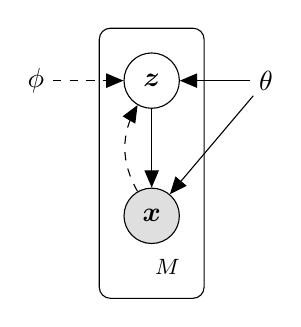
\begin{tikzpicture}
\tikzstyle{node}=[node distance=0.2cm and 0.2cm]
\node[latent] (z) {$\vz$};
\node[obs, below=of z] (x) {$\vx$};
\node[const, left=of z] (phi) {$\phi$};
\node[const, right=of z] (theta) {$\theta$};
\edge {z} {x} ; %
\path (x) edge[->, dashed, bend left] (z) ;%

\edge[shorten <=3pt, dashed] {phi} {z} ; %
\edge[shorten <=3pt] {theta} {z} ; %
\edge[shorten <=3pt] {theta} {x} ; %
\plate[inner sep=0.3cm] {M} {(z)(x)} {$M$}; %
\end{tikzpicture}
\caption{A graphical model of a VAE. The solid lines represent the generative process, and the dashed lines represent the inference process. The rectangular plate notation means we can sample M times from $\vz$ and $\vx$ while keeping $\theta$ fixed. The dashed lines denote the encoding process.}
\end{figure}

\begin{figure}
%\captionsetup{width=.8\linewidth}
\centering
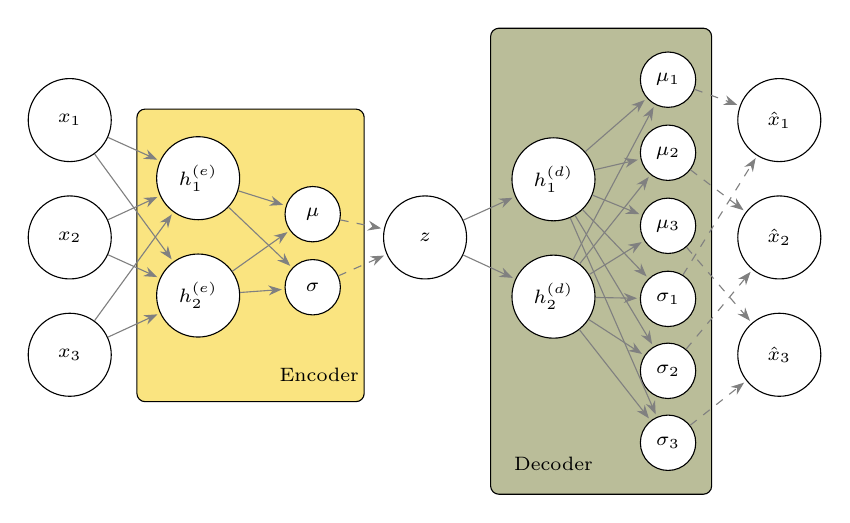
\begin{tikzpicture}[shorten >=1pt,->,draw=black!50, myarrow/.style={-Stealth}]
    \tikzstyle{every pin edge}=[<-,shorten <=1pt]
    \tikzstyle{neuron}=[circle,draw=black,fill=white!50,minimum size=\nodesize,inner sep=0pt,node distance=\nodesep and \layersep]
    \tikzstyle{input neuron}=[neuron];
    \tikzstyle{output neuron}=[neuron,minimum size=\smallnodesize,node distance=\smallnodesep and \layersep];
    \tikzstyle{hidden neuron}=[neuron];
    \tikzstyle{annot}=[text centered, node distance=0.4cm];

    \scriptsize
    % Draw the nodes
    \node[input neuron] (I-1) at (0,0) {$x_1$};
    \foreach \name [count=\i] in {2,3}
        \node[input neuron, below=of I-\i] (I-\name) {$x_{\name}$};

    \node[hidden neuron, right=of I-1, yshift=-0.5*\nodesize-0.5*\nodesep] (he-1) {$h^{(e)}_1$};
    \node[hidden neuron, below=of he-1] (he-2) {$h^{(e)}_2$};
        
    \node[output neuron, right=of he-1, yshift=-0.5*\smallnodesize-0.5*\smallnodesep] (eo-1) {$\mu$};
    \node[output neuron, below=of eo-1] (eo-2) {$\sigma$};

    \node[hidden neuron, right=of I-2, xshift=\nodesize+\smallnodesize+2*\layersep] (z) {$z$};
        
    \node[hidden neuron, right=of z, yshift=0.5*\nodesize+0.5*\nodesep] (hd-1) {$h^{(d)}_1$};
    \node[hidden neuron, below=of hd-1] (hd-2) {$h^{(d)}_2$};

    \node[output neuron, right=of hd-1, yshift=3*\nodesep / \smallnodesep *\smallnodesep] (do-1) {$\mu_1$};
    \foreach \name [count=\i] in {2,3}
        \node[output neuron, below=of do-\i] (do-\name) {$\mu_\name$};
   \foreach \name [count=\i] in {4,...,6}
        \node[output neuron, below=of do-3, yshift=\smallnodesize+\smallnodesep-\i*\smallnodesize - \i*\smallnodesep] (do-\name) {$\sigma_\i$};
        
    \foreach \name in {1,2,3}
        \node[hidden neuron, right=of I-\name, xshift=3*\nodesize+2*\smallnodesize+5*\layersep] (O-\name) {$\hat{x}_{\name}$};

    % Connect every node
    \foreach \source in {1,...,3}
        \foreach \dest in {1,...,2}
            \draw [myarrow] (I-\source) -- node[sloped] {} (he-\dest);
            
    \foreach \source in {1,...,2}
        \foreach \dest in {1,...,2}
            \draw [myarrow] (he-\source) -- node[sloped] {} (eo-\dest);
            
    \foreach \source in {1,...,2}
        \draw [myarrow,dashed] (eo-\source) -- node[sloped] {} (z);
    
    \foreach \dest in {1,...,2}
        \draw [myarrow] (z) -- node[sloped] {} (hd-\dest);

    \foreach \source in {1,...,2}
        \foreach \dest in {1,...,6}
            \draw [myarrow] (hd-\source) -- node[sloped] {} (do-\dest);

    \foreach \source in {1,...,3}
        \draw [myarrow,dashed] (do-\source) -- node[sloped] {} (O-\source);
    \foreach \source [count=\i] in {4,...,6}
        \draw [myarrow,dashed] (do-\source) -- node[sloped] {} (O-\i);

    \node[annot,right=of he-2, yshift=-1cm] (encoder) {Encoder};% $q\given{z}{x}$};
    \node[annot,below=of hd-2, yshift=-1cm] (decoder) {Decoder};% $p\given{\hat{x}}{z}$};

    \begin{scope}[on background layer]
        \draw[rounded corners=3pt,fill=curry!50]
            ($(he-1.north west)+(-0.4,0.5)$) rectangle ($(eo-2.south east)+(0.4,-1.2)$);
        \draw[rounded corners=3pt,fill=moss!50,label=left:ok]
            ($(do-1.north west)+(-2,0.4)$) rectangle ($(do-6.south east)+(0.3,-0.4)$);
    \end{scope}
\end{tikzpicture}
\caption{A variational autoencoder network with two layers in both the encoder and decoder and one latent variable $z$. Dashed arrows denote samples from probabilistic neurons, in this example both posterior and likelihood are Gaussian.}
\label{fig_gm_vae}
\end{figure}
The generative model maximizes Equation \ref{eq:maximize_vae}. If the choice of distribution is Gaussian, then
\begin{equation}
    p_{\theta}\given{\vx}{\vz} = \mathcal{N}\given{\vx}{f(\vz; \theta), \sigma^2 \times \mathbf{I}}
\end{equation}

That is, the likelihood $p_{\theta}\given{\vx}{\vz}$ has mean $\mu = f(\vz; \theta)$ and diagonal covariance $\Sigma = \sigma^2 \times \mathbf{I}$. This distribution can be modelled by a function approximator such as a neural network. If we model $p_{\theta}(\vz)$ as an uninformed Gaussian prior $\mathcal{N}(\boldsymbol{0}, \boldsymbol{I})$, we can take the gradient of the equation and and optimize it using gradient descent. However, it is generally intractable to simply sample from $\vz$ and compute $p(\vx) \approx \frac{1}{N}\sum_i^N p \given{\vx}{\vz^{(i)}}$ if $N$ is large. The reason for this is that for most $\vz^{(i)}$, $\ptheta \given{\vx}{\vz^{(i)}}$ will be very low, so the idea is to try to only sample instances of $\vz$ that are likely to have produced $\vx$.

As mentioned previously, we can approach this problem with a new function $\qphi \given{\vz}{\vx}$ that finds values of $\vz$ that are much more likely under $\qphi$ than under $\ptheta$. We can express the desire to have $\vz$ produced under $\qphi \given{\vz}{\vx}$ to be similar to those produced under $\ptheta \given{\vz}{\vx}$ using the Kullbach-Liebler (KL) divergence measure (dropping the indices $\theta, \phi$ for brevity)

\begin{equation}
\begin{split}
\KL{q \given{\vz}{\vx}}{p \given{\vz}{\vx}} &= \E_{q \given{\vz}{\vx} } \big [\log{q \given{\vz}{\vx}} - \log{p \given{\vz}{\vx}} \big ] \\
%- \int p \given{\vz}{\vx} \log{p \given{\vz}{\vx}}d\vz - \\
%& \quad \quad \big(- \int p \given{\vz}{\vx} \log{q \given{\vz}{\vx})}d\vz \big) \\
%\E_{q \given{\vz}{\vx} } \big [\log{q \given{\vz}{\vx}} - \log{p \given{\vz}{\vx}} \big ] \\
%&= \bigg{\{} \text{Expand $P(z|X)$ using Bayes' theorem \bigg{\}}} \\
%&= \E_{q \given{\vz}{\vx} }\big {[} \log{Q(z|X)} - \big{(} \log{P(X|z)} + \log{P(z)} - \log{P(X)} \big{)} \big{]}\\
&= \E_{q \given{\vz}{\vx} }\big {[} \log{q \given{\vz}{\vx})} - \overbrace{ \big{(} \log{p \given{\vx}{\vz}} + \log{p(z)} - \log{p(\vx)} \big{)} }^{\text{Expand $p\given{\vz}{\vx}$ using Bayes' theorem}} \big ]\\
&= \E_{q \given{\vz}{\vx} } \big{[} \log{q \given{\vz}{\vx}} - \log{p \given{\vx}{\vz}} - \log{p(\vz)} \big{]} + \log{p(\vx)} \\
&= \E_{q \given{\vz}{\vx} } \big{[} \KL{q \given{\vz}{\vx}}{p(\vz)} - \log{p \given{\vx}{\vz}} \big{]} + \log{p(\vx)}
\end{split}
\label{kl-eq}
\end{equation}

This gives the key equation to \vae{}s known as the Evidence Lower Bound (ELBO)

\begin{align}
%\log{P(X)} - D[Q(z|X) || P(z|X)] &= \E_{q \given{\vz}{\vx} } \big{[} \log{P(X|z)} + \log{P(z)} - \log{Q(z|X)} \big{]} \\
\nonumber \lefteqn{\log{\ptheta(\vx)} - \KL{\qphi \given{\vz}{\vx}}{\ptheta \given{\vz}{\vx}}} \\
& & & = \E_{\qphi \given{\vz}{\vx} } \big{[} \log{\ptheta \given{\vx}{\vz}} - \KL{\qphi \given{\vz}{\vx}}{\ptheta(\vz)} \big{]}
%\end{split}
\label{eq_vae}
\end{align}

Maximizing the left hand side of this equation means that we are maximizing $\log{\ptheta(\vx)}$ and subsequently minimizing an error term $\KL{\qphi \given{\vz}{\vx}}{\ptheta \given{\vz}{\vx}}$ since the KL divergence is always positive. The hope is that $\qphi \given{\vz}{\vx}$ will be very close to $\ptheta \given{\vz}{\vx}$, causing the divergence term to be zero, meaning we are directly optimizing $\log \ptheta(\vx)$. The right hand of the equation side looks much like an autoencoder. The first term can \emph{decode} $\vz$ into $\vx$, and the second term can \emph{encode} $\vx$ into $\vz$. This side of the equation can be optimized with gradient descent.

Now we just need to figure out how to model $\qphi$. A common choice is a Gaussian distribution, $\qphi \given{\vz}{\vx} = \mathcal{N}\given{\vz}{\mu (\vx;\phi), \Sigma(\vx; \phi)}$, where $\phi$ are parameters learned from the data. This results in a KL divergence term that can be computed in closed form:

\begin{align}
\nonumber \lefteqn{\KL{\mathcal{N}(\mu_0, \Sigma_0)}{\mathcal{N}(\mu_1, \Sigma_1)} =} \\
& & \frac{1}{2} \bigg{(} \text{tr}(\Sigma_1^{-1}\Sigma_0) + (\mu_1 - \mu_0)^\top)\Sigma_1^{-1}(\mu_1 - \mu_0) - k - \log \frac{\det \Sigma_1}{\det \Sigma_0}) \bigg{)}
\label{kl-closed-form-eq1}
\end{align}

where $k$ is the dimension of the vector space. This is simplified if we assume an uninformative prior:

\begin{align}
\nonumber \lefteqn{ \KL{\mathcal{N}(\mu (\vx; \phi), \Sigma (X; \phi)}{ \mathcal{N}(\vec{0}, \vec{I})} =}\\
& & \frac{1}{2} \bigg{(} \text{tr}(\Sigma (\vx; \phi)) + \mu (\vx; \phi)^\top \mu (\vx; \phi) - k - \log{\det{\Sigma (\vx; \phi)}} \bigg{)}
\label{kl-closed-form-eq2}
\end{align}

The idea is to sample $\vz$ from $\qphi \given{\vz}{\vx}$ and compute $\log{ p_\theta \given{\vx}{\vz}}$ as an approximation of $\E_{\vz \sim \qphi} [\,\log{\ptheta \given{\vx}{z}}\,]$. The output of the encoder network $\qphi$ is a probability distribution, such as the mean and covariance of a Gaussian distribution $\vec{z} \sim \mathcal{N}\big(\mu_{\vz} (\vx; \phi), \Sigma_{\vz} (\vx; \phi)\big)$. However, stochastic units inside the network are not differentiable, and thus it is not possible to backpropagate the error with respect to the parameters of the distribution.

To solve the problem of non-differentiable units, \parencite{kingma2013auto} suggested a ''trick'' that splits up the network into two parts. We sample an auxiliary variable $\epsilon = \N(\vec{0}, \vec{I})$ and reparameterize $\vz$ with a deterministic function $\vz=g(\vx, \epsilon)$. Assuming a Gaussian distribution over $\vz$, a valid reparameterization is $g(\vx, \epsilon) = \mu(\vx; \phi) + \Sigma(\vx; \phi) \times \epsilon$.
Thus, we treat the stochastic $\epsilon$ as input which allows backpropagation with gradient descent and maximum likelihood estimates for $\phi$.
%This means we can compute $\mathop{\mathbb{E}}_{\qphi \given{\vz}{\vx} } P(X|z,\theta)$ and simply need to find a way to make it as similar  


\subsection{Conditional Variational Autoencoder}

The Conditional Variational Autoencoder (\cvae{}) is a modification to the original \vae{} which allows for a deep conditional generative model. The \cvae{} models a distribution of the output space as a generative model conditioned on the the input observation. This is done by modulating the prior on the latent variables.

The \cvae{} has a very similar structure to the \vae{} with a recognition network $\qphi \given{\vz}{\vx, \vy}$, a prior $\ptheta \given{\vz}{\vx}$ and a generative network $p_{\theta}\given{\vy}{\vx, \vz}$. The generative process is as follows: for input $\vx$, we sample from the prior distribution $\ptheta \given{\vz}{\vx}$ to generate the output $\vy$ from the distribution $\ptheta \given{\vy}{\vx, \vz}$.

%The generative process of of the \cvae{} is to draw $\vz$ given the input $\vx$ from the prior distribution $p_{\theta}\given{\vz}{\vx}$, and the output is generated from a distribution $p_{\theta}\given{\vy}{\vx, \vz}$.

%\subsection*{Variational lower bound of conditional log-likelihood}
The variational lower bound for \cvae{} with the new output variable $\vy$ is reformulated as follows:

\begin{equation}
\begin{split}
\log p_{\theta}\given{\vy}{\vx} &= \KL{q_{\theta}\given{\vz}{\vx, \vy}}{p_{\theta}\given{\vz}{\vx}} + \E{}_{q_{\phi}\given{\vz}{\vx, \vy}} \big [ - \log q_{\phi}\given{\vz}{\vx, \vy} + \log p_{\theta}\given{\vy, \vz}{\vx} \big ]
\\
&\geq \E{}_{q_{\phi}\given{\vz}{\vx, \vy}} \big [ - \log q_{\phi}\given{\vz}{\vx, \vy} + \log p_{\theta}\given{\vy}{\vx, \vz} \big ]
\\
&= \E{}_{q_{\phi}\given{\vz}{\vx, \vy}} \big [ - \log q_{\phi}\given{\vz}{\vx, \vy} + \log p_{\theta}\given{\vz}{\vx} \big ] + \E{}_{q_{\phi}\given{\vz}{\vx, \vy}} \big [ \log p_{\theta} \given{\vy}{\vx, \vz} \big ]
\\
&= -\KL{q_{\phi}\given{\vz}{\vx, \vy}}{p_{\theta}\given{\vz}{\vx}} + \E{}_{q_{\phi}\given{\vz}{\vx, \vy}} \big [ \log p_{\theta} \given{\vy}{\vx, \vz} \big ]
\label{eq_cvae}
\end{split}
\end{equation}

% \subsection{VAE latent spaces}
% \subsubsection{Disentanglement with VAE}


%\subsection*{Learning to predict structured output}

In general, \vae{}s are used to \emph{autoencode} its input, and maximizing the ELBO is effective in training deep generative models. However, the same training may not be suitable to predict structured output for a \cvae{}. This is because during training of the \cvae{}, the output $\vy$ is fed as input to the encoder $q_{\theta}\given{\vz}{\vx, \vy}$. As such, the objective during training can be seen as a \emph{reconstruction} of $\vy$. However, during testing or inference, it uses the prior network $p_{\theta}\given{\vz}{\vx}$ to draw samples $\vz$ and \emph{predict} $\vy$. Prediction is considered a harder problem than reconstruction \parencite{Sohn2015}. Sohn et al discuss allocating more weight on the negative KL divergence term in the objective to reduce the gap between the latent encoding during training and testing. They find that this does not yield good results and instead propose to train the \cvae{} in a way that makes the predictions consistent during training and testing. This proposal introduces a objective for a model they call \emph{Gaussian Stochastic Neural Network} (GSNN).


\begin{equation}
\begin{split}
\mathcal{L}_{\text{GSNN}}(\vx, \vy, \vth, \vph) = \frac{1}{N} \sum_{n=1}^N \log p_\theta \given{\vy}{\vx, \vz^{(n)}}
\\
\vz^{(n)} = g_{\theta}(\vx, \epsilon^{(n)}), \epsilon^{(n)} \sim \mathcal{N}(\pmb{0}, \mathbf{I})
\end{split}
\end{equation}
This is then combined with the standard \cvae{} objective to form a hybrid objective with a scaling term $\alpha$:
\begin{equation}
\mathcal{L}_{\text{hybrid}} = \alpha \mathcal{L}_{\text{CVAE}} + (1 - \alpha) \mathcal{L}_{\text{GSNN}}
\end{equation}

\section{Transfer learning and sim-to-real}
\subsection{Domain and dynamics randomization}

A simple but powerful approach to transferring RL policies from simulation to the real world is to introduce uncertainty during training. The purpose is to provide enough simulated variability during training such that at test time the model is able to generalize to real-world data. Uncertainty can be applied to the dynamics of the system \parencite{Antonova2017}\parencite{peng} or the domain itself \parencite{tobin}. Both approaches attempt to reduce the discrepancies between simulation and the real world in order to produce more robust policies that learn to generalize to the domain and dynamics of the real world without physically training in it. 

By introducing random noise to the parameters of the simulator that affect the dynamics of the system during training, \parencite{Antonova2017} and \parencite{peng} show that it is possible to develop policies that are capable of adapting to very different dynamics, even including ones that differ significantly from the dynamics on which the policies were trained.

The approach by \parencite{tobin} is similar and focuses on randomizing the domain rather than the dynamics. In their work, they train using images as input and randomize the rendering of the simulator. This randomization includes colors and textures of objects, position and orientation of the camera, number of lights in the scene and the type and amount of random noise added to the images.

\subsection{Approaches for Sim-to-Real adjustment}
\todo[inline]{Write this.}
\subsubsection*{MAML}

\subsubsection*{Progressive nets}
Tries to address data efficiency.

Mention Elastic weight consolidation but doesn't address data efficiency.
\subsubsection*{Closing the Sim-to-Real Loop}
Not training a neural net to match. They're using simulator as a black box. Can utilize extra latent space when training on real data. det2stoc can be extended with extra latent varaibles after det2stoc



% \chapter{Related work}
% \label{relatedwork}

%The work completed as part of the thesis project touches on two topics: the task of system identification and Sim-to-Real transfer. None of the mentioned topics are considered solved problems and are the subject of intense research. This chapter briefly summarizes the work done in each of these domains and discusses the benefits and drawbacks of available solutions.



% \section{Semi/fully labeled to provide supervision for encoding latent variables}

% In semi-supervised learning, both labeled examples from p(x,y) and unlabeled from p(x) are used to estimated p(y|x). The goal is to learn a representation so that examples from the same class have similar representations. If the examples cluster tightly in the input space they should be mapped to similar representations.



\chapter{Methods}
\label{methods}

This chapter describes the motivation behind the proposed \dettostoc{}, and outlines the algorithm in detail including the network architecture.

\section{Motivation}

%Combining deep learning with physics-based modeling has several positive benefits.  

Consider a physics simulator that correctly describes a dynamical system using laws of physics and mathematics. Since neural networks learn from experience, it is possible to learn the dynamics of this system and make accurate predictions given enough input and output samples. According to the universal approximation theorem, a neural network with at least one hidden layer with a nonlinear activation function can approximate any smooth function with sufficient accuracy provided that there are enough hidden units in the layer \parencite{Hornik1989} \parencite{Cybenko1989}.

%These networks are thus universal approximators, in their mapping of input vectors to output vectors, which is what makes them so useful for tasks in artificial intelligence. On the other hand, the sufficient number of hidden units of [26] is not guaranteed to be manageable computationally [27]. As is pointed out by Lin et al. in [27], the reason that a lot of neural network function approximations however indeed seem to work for a variety of tasks [25] is that the class of functions we are actually interested in is tiny, and essentially of low dimensionality, compared to the total collection of estimable functions.

General-purpose simulators like MuJoCo employ efficient dynamics models to make approximations but do not explicitly model uncertainty. MuJoCo is fast, however, in complex scenarios it is still time consuming to compute frictional contacts. In contrast, a forward pass in a neural network is fast, and a hybrid solution that combines deterministic simulators with learnable, stochastic neural networks allows for models that are efficient, expressive and generalizable.

%information from observed data, for example when there are unknown variables or parameters that cannot be measured, but we have observed data on how the system behaves.

The basic idea of this work is to train a \cvae{} using real data to produce a stochastic simulator, but as mentioned previously, this is not data-efficient. So, instead of starting from random encoder and decoder weights, we will first align the decoder function $\fdecoder{}$ with the output of an existing general-purpose simulator $\fsimulator{}$.

Furthermore, real data comes with uncertainty. This uncertainty can be modelled with a generative model such as a \vae{}, and the slightly modified \cvae{} allows us to condition on current state. Moreover, we can use our prior knowledge in a bayesian manner to reason about sensible values that affect the environment.

Domain and dynamics randomization are powerful techniques to reduce the reality gap. However, as shown with experiments in \parencite{Chebotar2018}, using wide distribution for randomization can cause infeasible solutions that hinder policy learning, or sub-optimal and conservative policies. Instead of adding noise to observations, we introduce noise during simulation by collecting a set of trajectories using a range of simulation parameters $\psi$. 

%Prior knowledge (parameters to affect environment) pre training

\section{Proposed \dettostoc{} algorithm}
\label{det2stoc:algorithm}

Our approach specifies how existing general-purpose simulators could be used to make the learning of the stochastic function $g(\cdot)$ more data efficient. We denote real observations $\trajreal$ and simulated observations parameterized by $\vpsi$ $\trajsim_{\vpsi}$. Algorithm \ref{alg:det2stoc} describes \dettostoc{} procedure.

\vspace{\baselineskip}% Insert a blank line
\begin{algorithm}[H]
%  \LinesNumberedHidden
  \DontPrintSemicolon
  $\trajreal \leftarrow$ collect real trajectories \; \label{det2stoc:step1}
  $\vpsi_0 \leftarrow$ initialize sim parameters \;
  \For{i $\in \{0, ..., N\}$}{
    $\trajsim_{\vpsi_i} \leftarrow$ collect sim trajectories from $\fsimulator{}(\vpsi_{i})$ \;
    %$\fdecoder{} \xleftarrow{}$ PreTrain($\trajsim$, $\vpsi_i$) \;
    $\ptheta \leftarrow$ train \fdecoder{} on $\trajsim_{\vpsi_i}$\;% \ptheta \given{\vns}{\vpsi_i, \vs, \va}$ \;
    %$f^{\cvae{}} \xleftarrow{}$ Train($\trajreal, \fdecoder{}$) with \fdecoder{} frozen\;
    $\qphi \leftarrow$ train \cvae{} on $\trajreal$ using frozen $\fdecoder{}$\;
    $\vph_{\mu, \sigma} \leftarrow$ compute posterior $\qphi$ given $\trajreal$\;% $\qphi \given{\vz}{\vs, \va, \vns} $\;%($\trajreal, f^{\cvae{}}$) \;
    $\vpsi_{i+1} \xleftarrow[]{} \vph_{\mu, \sigma}$ \;
    %update parameter distribution from posterior given $\trajreal$ \;
  } % end for N robot trials
  \caption{det2stoc}
  \label{alg:det2stoc}
\end{algorithm}
\vspace{\baselineskip}% Insert a blank line
First, we collect trajectories $\trajreal$ from our real environment.
Then, we choose a set of initial parameters that cannot be measured or that have uncertainty associated with them. We decide on an initial distribution $\vpsi_0$ for these parameters, typically an uninformative distribution, for example a uniform distribution or a wide truncated Gaussian distribution.
In the beginning of each iteration $i$, we run simulations parameterized by samples from $\vpsi_i$ and collect trajectories $\trajsim_{\vpsi_i}=\{\vs, \va, \vns\}^{1:N}$. The decoder network $\fdecoder{}$ is pre-trained separately on the simulated data $\trajsim_{\vec{\psi_i}}{}$ to match $\fsimulator(\vpsi_i)$ using a negative log likelihood loss function. However, during this pre-training phase, instead of sampling $\vz$ from the posterior $\qphi$, the network is fed parameters $\vpsi$ used during simulation for that particular timestep $\fdecoder = f(\vpsi; \vth)$. The intention of this step is to train the decoder to capture how the simulation parameters $\vpsi$ affect the system dynamics.% which will infer parameters $\vpsi_{\mu,\sigma}$ that closely ressemble those of real-world dynamics.
The \cvae{} is subsequently trained to match $\fpsisimulator{}$, but the decoder weights are kept frozen. The purpose of this step is to train the encoder to produce a posterior that maximizes the log likelihood of the next state $\vns$, while ensuring that the decoder does not catastrophically forget \parencite{French2006CatastrophicFI} what it learned during pretraining. The input to the encoder is state $\vs$, action $\va$ and next state $\vns$. %Including the next state ensures that there is enough information for the network to infer what parameter corresponds to which output.
Finally, we update our parameters $\vpsi_{i+1}$ with the posterior $\vph_{\mu, \sigma}$.

This process can be repeated multiple times. The result of the \dettostoc{} algorithm is the trained decoder as well as the learned $\vph_{\mu, \sigma}$. Because of how the training procedure was set up, the network is now aligned with real world data.

%Since the \cvae{} includes the target $\vy$ in the posterior formulation, and we have trained the \cvae{} in a way that it is encouraged to represent the simulator parameters in latent space, we can perform system identification using variational inference and sampling from the posterior $q_{\vth} \given{\vz}{\vx,\vy}$. The idea is that if the \cvae{} has been trained on sufficiently many samples, it should be able to produce a posterior that in fact matches the parameter value that best predict the next state $\vns$.

\begin{figure}
\centering
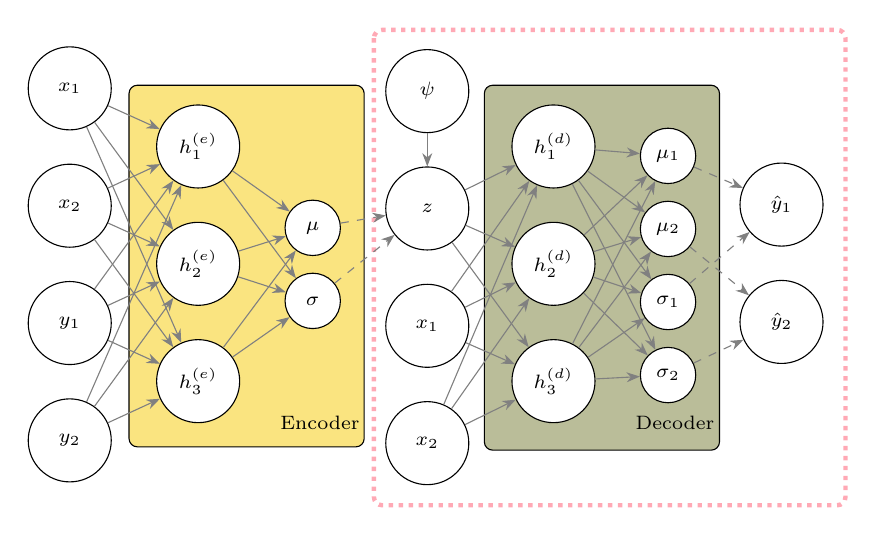
\begin{tikzpicture}[shorten >=0pt,-,draw=black!50, node distance=\nodesep and \layersep, myarrow/.style={-Stealth}]
    \tikzstyle{every pin edge}=[<-,shorten <=0pt]
    \tikzstyle{neuron}=[circle,draw=black,fill=white!50,minimum size=30pt,inner sep=0pt]
    \tikzstyle{probabilistic neuron}=[neuron,minimum size=\smallnodesize,node distance=\smallnodesep and \layersep]
    \tikzstyle{input neuron}=[neuron];
    \tikzstyle{output neuron}=[probabilistic neuron];
    \tikzstyle{hidden neuron}=[neuron];
    \tikzstyle{annot}=[text centered, node distance=0.8cm];
    \tikzstyle{myarrow dasharrow}=[myarrow dashed];
    \scriptsize
    % Draw the nodes
    \node[input neuron] (I-1) at (0,0) {$x_1$};
    \node[input neuron, below=of I-1] (I-2) {$x_2$};
    \node[input neuron, below=of I-2] (I-3) {$y_1$};
    \node[input neuron, below=of I-3] (I-4) {$y_2$};
        
    \node[hidden neuron, right=of I-1, yshift=-0.5*(\nodesep+\nodesize)] (he-1) {$h^{(e)}_1$};
    \node[hidden neuron, below=of he-1] (he-2) {$h^{(e)}_2$};
    \node[hidden neuron, below=of he-2] (he-3) {$h^{(e)}_3$};
        
    \node[probabilistic neuron, right=of he-2, yshift=0.5*(\smallnodesize+\smallnodesep)] (mu) {$\mu$};
    \node[probabilistic neuron, below=of mu] (sigma) {$\sigma$};
        
    %\foreach \name / \y in {1,...,2}
    \node[hidden neuron, right=of mu, yshift=0.5*(\smallnodesize-\smallnodesep)] (z-1) {$z$};
    
    \node[hidden neuron, above=of z-1] (psi-1) {$\psi$};

    \node[input neuron, below=of z-1] (c-1) {$x_1$};
    \node[input neuron, below=of c-1] (c-2) {$x_2$};

    \foreach \name in {1,...,3}
        \node[hidden neuron, right=of he-\name, xshift=2*\layersep + \nodesize+\smallnodesize] (hd-\name) {$h^{(d)}_\name$};

    \node[probabilistic neuron, right=of hd-2, yshift=1.5*(\smallnodesize+\smallnodesep] (O-1) {$\mu_1$};
    \node[probabilistic neuron, below=of O-1] (O-2) {$\mu_2$};
    \node[probabilistic neuron, below=of O-2] (O-3) {$\sigma_1$};
    \node[probabilistic neuron, below=of O-3] (O-4) {$\sigma_2$};

    \node[input neuron, right=of hd-1, xshift=\layersep+\smallnodesize, yshift=-0.5*(\nodesize+\nodesep)] (Y-1) {$\hat{y}_1$};
    \node[input neuron, below=of Y-1] (Y-2) {$\hat{y}_2$};

    % Connect every node
    \foreach \source in {1,...,4}
        \foreach \dest in {1,...,3}
            \draw [myarrow] (I-\source) -- node[sloped] {} (he-\dest);
            
    \foreach \source in {1,...,3}
        \foreach \dest in {mu, sigma}
            \draw [myarrow] (he-\source) -- node[sloped] {} (\dest);

    \foreach \source in {mu, sigma}
            \draw [myarrow,dashed] (\source) -- node[sloped] {} (z-1);

    \foreach \source in {1,...,1}
        \foreach \dest in {1,...,3}
            \draw [myarrow] (z-\source) -- node[sloped] {} (hd-\dest);

    \foreach \source in {1,...,3}
        \foreach \dest in {1,...,4}
            \draw [myarrow] (hd-\source) -- node[sloped] {} (O-\dest);

    \foreach \source in {1,...,2}
        \foreach \dest in {1,...,3}
            \draw [myarrow] (c-\source) -- node[sloped] {} (hd-\dest);
            
    \foreach \source in {1,3}
        \draw [myarrow,dashed] (O-\source) -- node[sloped] {} (Y-1);
           
    \foreach \source in {2,4}
        \draw [myarrow,dashed] (O-\source) -- node[sloped] {} (Y-2); 
            
    \draw [myarrow] (psi-1) -- node[sloped] {} (z-1);

    % Annotate the layers
    \node[annot, below right=of he-3, yshift=0.6cm] (encoder) {Encoder};% $q\given{z}{x}$};
    \node[annot, below right=of hd-3, yshift=0.6cm] (decoder) {Decoder};% $p\given{\hat{x}}{z}$};
    
    \begin{scope}[on background layer]
        %\path[use as bounding box] (0,0) rectangle (10,10);
        \draw[rounded corners=3pt,fill=curry!50]
            ($(he-1.north west)+(-0.5,0.4)$) rectangle ($(sigma.south east)+(0.4,-1.6)$);
        \draw[rounded corners=3pt,fill=moss!50]
            ($(hd-1.north west)+(-0.5,0.4)$) rectangle ($(O-4.south east)+(0.4,-0.7)$);
        \draw[rounded corners=3pt,draw=rose!100,ultra thick,dotted]
            ($(psi-1.north west)+(-0.3,0.4)$) rectangle ($(O-4.south east)+(2,-1.4)$);
            
        % \draw[rounded corners=3pt,draw=black!100, thick]
        %     ($(O-1.north west)+(-0.4,0.4)$) rectangle ($(O-2.south east)+(0.4,-0.4)$);
        % \draw[rounded corners=3pt,draw=black!100, thick]
        %     ($(O-3.north west)+(-0.4,0.4)$) rectangle ($(O-4.south east)+(0.4,-0.4)$);
            
        % \draw[rounded corners=3pt,draw=black!100, thick]
        %     ($(mu.north west)+(-0.4,0.4)$) rectangle ($(mu.south east)+(0.4,-0.4)$);
        % \draw[rounded corners=3pt,draw=black!100, thick]
        %     ($(sigma.north west)+(-0.4,0.4)$) rectangle ($(sigma.south east)+(0.4,-0.4)$);
    \end{scope}
    
    %\node[annot, above=of decoderbox] {okokok};
\end{tikzpicture}
\caption{The \dettostoc{} architecture with a simple network consisting of a 2D vector of inputs $\vec{x}$ and a 2D target vector $\vec{y}$. Dashed arrows denote sampling from probabilistic neurons. The dotted line shows the decoder pre-training phase where $\vpsi$ replaces samples from the posterior.}
\label{fig:det2stoc_architecture}
\end{figure}

\section{Conditioning architecture and transfer-aware training}

\subsection{Network and training parameters}
Both the encoder and decoder networks consist of a 3-layer network with 64 units using ReLU activations and layer normalization \parencite{Ba2016}. The number of latent variables is equal to the number of variable parameters used when collecting the training data from simulation. The output from the encoder and decoder networks are multivariate normal distributions with diagonal covariance matrices.

A common problem during training of a \vae{} is latent variable collapse. When this phenomenon occurs, the \vae{} learns a good generative model of the data but does not learn good representations of the individual data points. Specifically, when maximizing the lower bound of the log marginal likelihood, the posterior ''collapses'' at inference, when the posterior is set equal to the prior, essentially when the posterior is independent of the data. We combat this problem with skip-connections from the posterior to the decoder, essentially enforcing a stronger connection between the latent variables and the likelihood function \parencite{Dieng2018}.

Since the \cvae{} has the target $\vy$ in its posterior formulation, it is prone to overfitting unlike a regular \vae{} which tends to be regularized by the KL divergence term in the ELBO. The authors of \parencite{Sohn2015} suggest adding dropout to the encoder to combat this problem. A dropout rate of $0.5$ is used on the input layer to the encoder and helped avoiding extremely peaked latent encodings.

A learning rate of $1e^{-4}$ with a cosine decay is used to minimize the loss function using Adam \parencite{kingma2014adam}. We also employed early stopping for all parts of the training.

\section{Implementation details}

Since the KL divergence term in the objective function penalizes priors that diverge from the standard normal distribution, the simulator parameters are translated and scaled to have a mean of 0 and standard deviation of 1:

\begin{equation*}
    z = \frac{x - \mu}{\sigma}
\end{equation*}

Rather than trying to output the next state, the target $\vy$ is the delta between next and current state:

\begin{equation*}
    \vy_{\Delta} = \vns - \vs
\end{equation*}

\subsection{Tools}

The implementation was done in Python 3.5.2. Neural networks were built using TensorFlow \parencite{tensorflow2015-whitepaper}. 
All experiments were conducted on a machine with a Intel Core i7-8700 CPU, NVIDIA GeForce 1080Ti and 16GB of RAM.

\chapter{Experimental results}
\label{experiments}

This chapter introduces in greater detail the data and results for the thesis project. We perform three experiments. The first is an analytic experiment, constructed as a proof of concept to confirm the basic premise that the \cvae{} can be used to predict conditional probabilities. In the following experiments we evaluate the \dettostoc{} algorithm in two different scenarios using MuJoCo.

Some questions we want to answer: How does \dettostoc{} compare against a baseline that has only trained on \emph{real} data? How many iterations of \dettostoc{} are required for \fdecoder{} to match \fsimulator{} with sufficient accuracy?


\section{Analytic experiment}
\label{exp:analytic}
As an initial experiment we use data with known distributions that can easily be analyzed. We define a joint distribution $p(s,a,s')$ and then attempt to learn the conditional distribution $p\given{s'}{s,a}$. If the distribution is a multivariate Gaussian, then the conditional distribution is also Gaussian and we can find analytic expressions for its mean and covariance. In the general case, if $\vec{Z}$ is a multivariate Gaussian variable of dimension $l+m$, we can partition $\vec{Z}$ into two multivariate variables $\vec{X}$ and $\vec{Y}$

\begin{equation}
\vec{Z} = 
\begin{bmatrix}
\vec{X} \\
\vec{Y}
\end{bmatrix}
\quad
\text{with sizes:} 
\begin{bmatrix}
l \\
m
\end{bmatrix}
\end{equation}
We then find their mean and covariance
\begin{equation}
\mu_{Z} = 
\begin{bmatrix}
\mu_{X} \\
\mu_{Y}
\end{bmatrix}
\quad
\text{with sizes:} 
\begin{bmatrix}
l \\
m
\end{bmatrix}
\end{equation}

\begin{equation}
\Sigma_{Z} = 
\begin{bmatrix}
\Sigma_{XX} & \Sigma_{XY} \\
\Sigma_{YX} & \Sigma_{YY}
\end{bmatrix}
\quad
\text{with sizes:} 
\begin{bmatrix}
l\times l & l \times m\\
m \times l & m \times m
\end{bmatrix}
\end{equation}
\\
The conditional distribution $p\given{\mathbf{X}}{\mathbf{Y}=\mathbf{y}}$ is then found by $\mathcal{N} (\mu_{\given{X}{Y}}, \Sigma_{\given{X}{Y}})$ where
\begin{align}
%\E[X \vert Y = y]
\mu_{\given{X}{Y}} &= \mu_{X} + \Sigma_{XY}\Sigma_{YY}^{-1}(y - \mu_{Y})
\label{eq_cond_mean}
\\
%Cov[X \vert Y = y]
\Sigma_{\given{X}{Y}} &= \Sigma_{XX} - \Sigma_{XY}\Sigma_{YY}^{-1}\Sigma_{YX}
\label{eq_cond_var}
\end{align}

The question is now is to see if it is possible to learn $\mu_{\given{X}{Y}}$ and $\Sigma_{\given{X}{Y}}$ using a \cvae{}.

% \begin{figure}
% \begin{center}
% 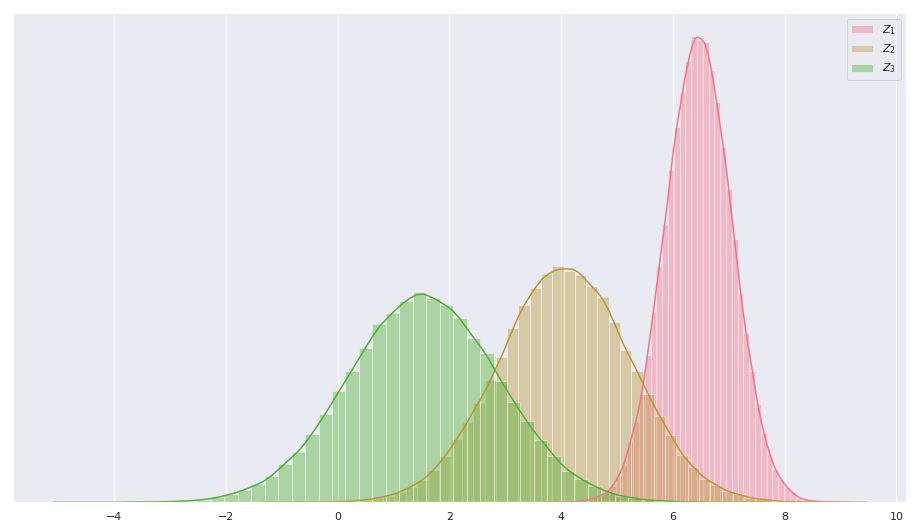
\includegraphics[width=0.8\textwidth]{img/trivariate}
% \caption{Example showing density for each univariate distribution given samples from a trivariate distribution $p(s, a, s')$.}
% \end{center}
% \end{figure}

\subsection{Training procedure}

To setup this experiment, we randomly generate the parameters of a trivariate normal distribution and ensure the covariance matrix is positive semi-definite. The \cvae{} is trained with samples from the trivariate distribution in the following way:

First, we sample $(s, a, s')$ from the trivariate distribution. Then, the probabilistic encoder is used to produce $\qphi \given{z}{s', s, a}$. We then modulate the posterior $z$ with the conditional input $s, a$ and use the decoder to predict the distribution $\ptheta \given{s'}{z, s, a}$. We can view this as analogous to the goal of learning the next state $s'$ conditioned on the current state $s$ and control actions $a$.

\begin{figure}
\centering
\captionsetup{size=footnotesize}
\begin{subfigure}{\linewidth}
  \centering
  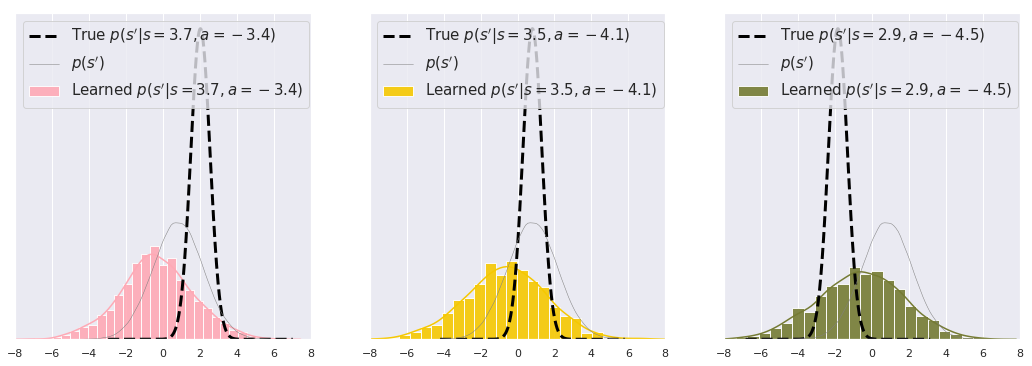
\includegraphics[width=1.0\linewidth]{img/trivariate/trivariate-epoch0}
  \caption{0 gradient steps}
  \label{fig_3_parameters_0}
\end{subfigure}
% \begin{subfigure}{\linewidth}
%   \centering
%   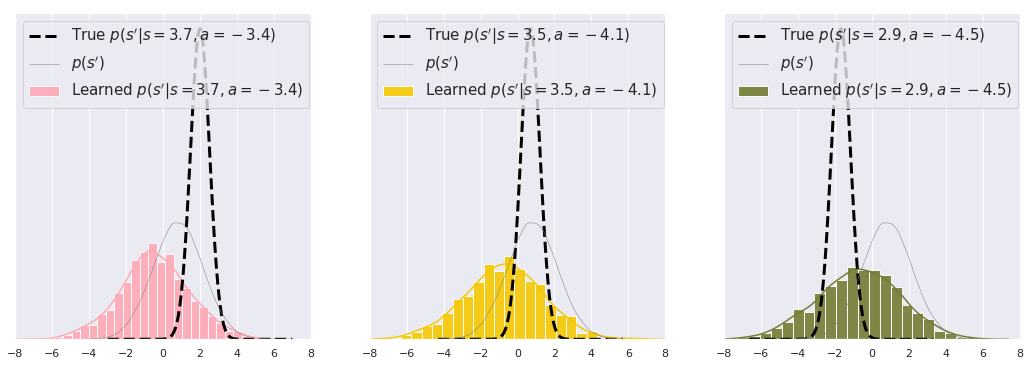
\includegraphics[width=1.0\linewidth]{img/trivariate/trivariate-epoch100}
%   \caption{100 gradient steps}
%   \label{fig_3_parameters_0}
% \end{subfigure}
\begin{subfigure}{\textwidth}
  \centering
  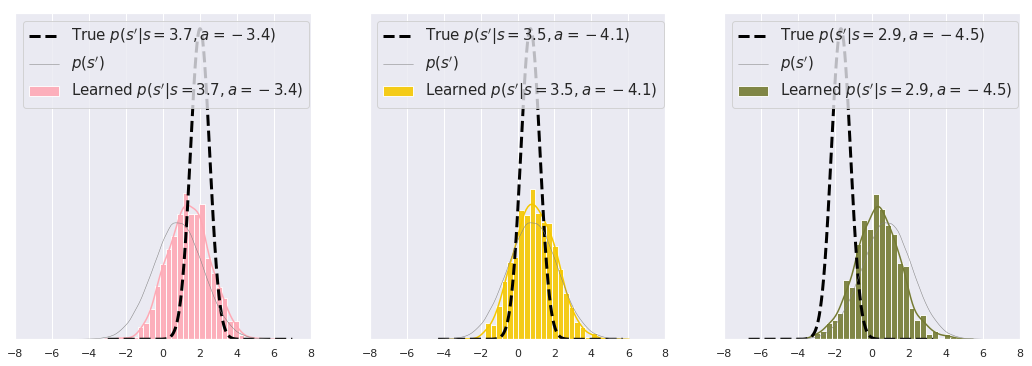
\includegraphics[width=1.0\linewidth]{img/trivariate/trivariate-epoch200}
  \caption{200 gradient steps}
\end{subfigure}
\begin{subfigure}{\textwidth}
  \centering
  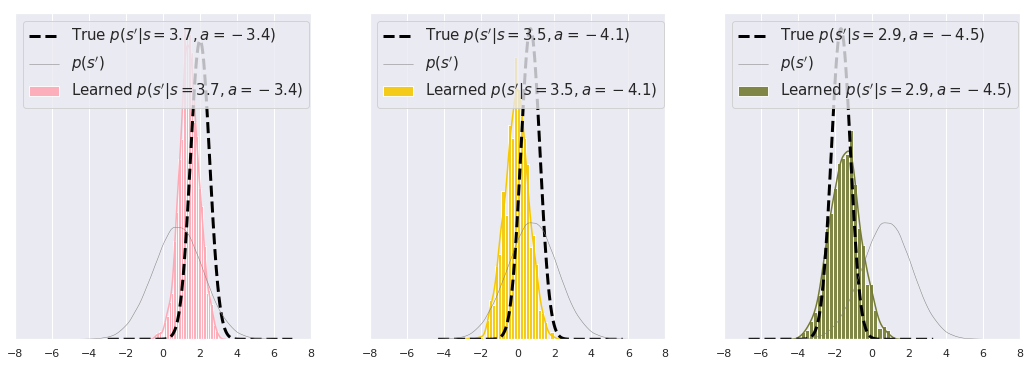
\includegraphics[width=1.0\linewidth]{img/trivariate/trivariate-epoch500.png}
  \caption{500 gradient steps}
\end{subfigure}
\begin{subfigure}{\textwidth}
  \centering
  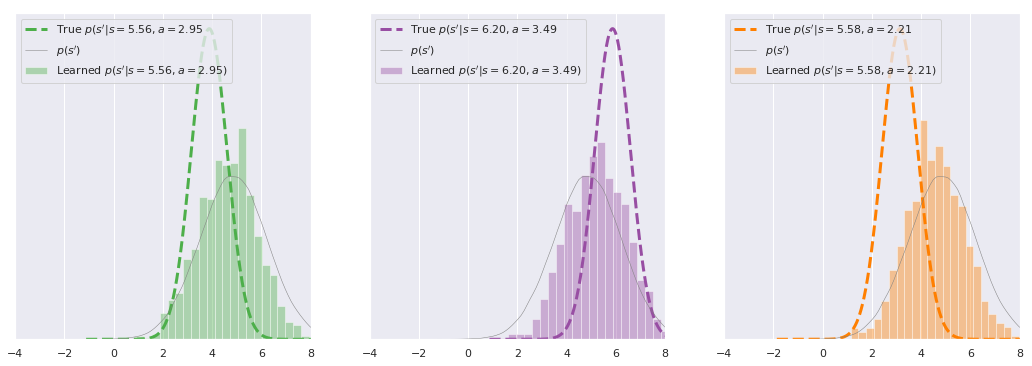
\includegraphics[width=1.0\linewidth]{img/trivariate/trivariate-epoch2000}
  \caption{2000 gradient steps}
\end{subfigure}

\caption[]{Three different density estimations during training for \ensuremath{p \given*{s'}{a,s}} where $a$ and $s$ have been randomly sampled from a known trivariate distribution in each plot and drawn as vertical lines. The expected density $p \given{s'}{s, a} \sim \N (\mu_{\given{s'}{s,a}}, \Sigma_{\given{s'}{s,a}})$ is computed and its outline plotted in thick dashed lines using equations \ref{eq_cond_mean} and \ref{eq_cond_var}.}
\label{fig:trivariate_density}
\end{figure}

As illustrated by Figure \ref{fig:trivariate_density}, the \cvae{} initially learns the distribution $p(s')$ but ultimately converges towards the conditional distribution $p \given{s'}{s, a} \sim \N (\mu_{\given{s'}{s,a}}, \Sigma_{\given{s'}{s,a}})$ after training on enough samples. %That is, the \cvae{} begins learning by ignoring the condition $s, a$, and instead memorizes the distribution $p(s')$, but after seeing enough samples it eventually learns to consider the condition and accurately predicts the conditional distribution $p \given{s'}{s, a}$.

\iffalse
\begin{figure}
\begin{center}
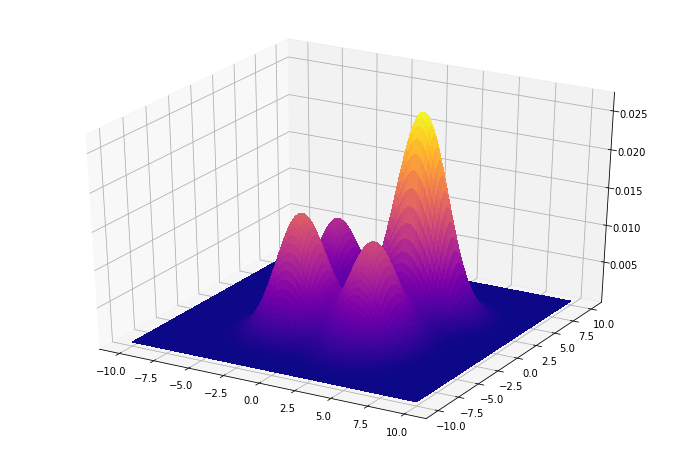
\includegraphics[width=8cm]{img/multimodal_bivariate_3d.png}
\caption{A multimodal mixture of bivariate Gaussians.}
\label{fig_multimodal_bivariate_3d}
\end{center}
\end{figure}
While this indicates that the \cvae{} can learn a conditional distribution, this does not demonstrate that the \cvae{} is capable of learning a multimodal distribution. So as another experiment, we model a bivariate mixture distribution seen in figure \ref{fig_multimodal_bivariate_3d}.

Interestingly, experiments show that increasing the size of the latent space results in a biased distribution that has one mode, rather than being multimodal. Furthermore, even without a mixture model, the \cvae{} can represent multimodal distributions. Results can be seen in figure \ref{fig_multimodal_bivariate}.

\begin{figure}
\begin{center}
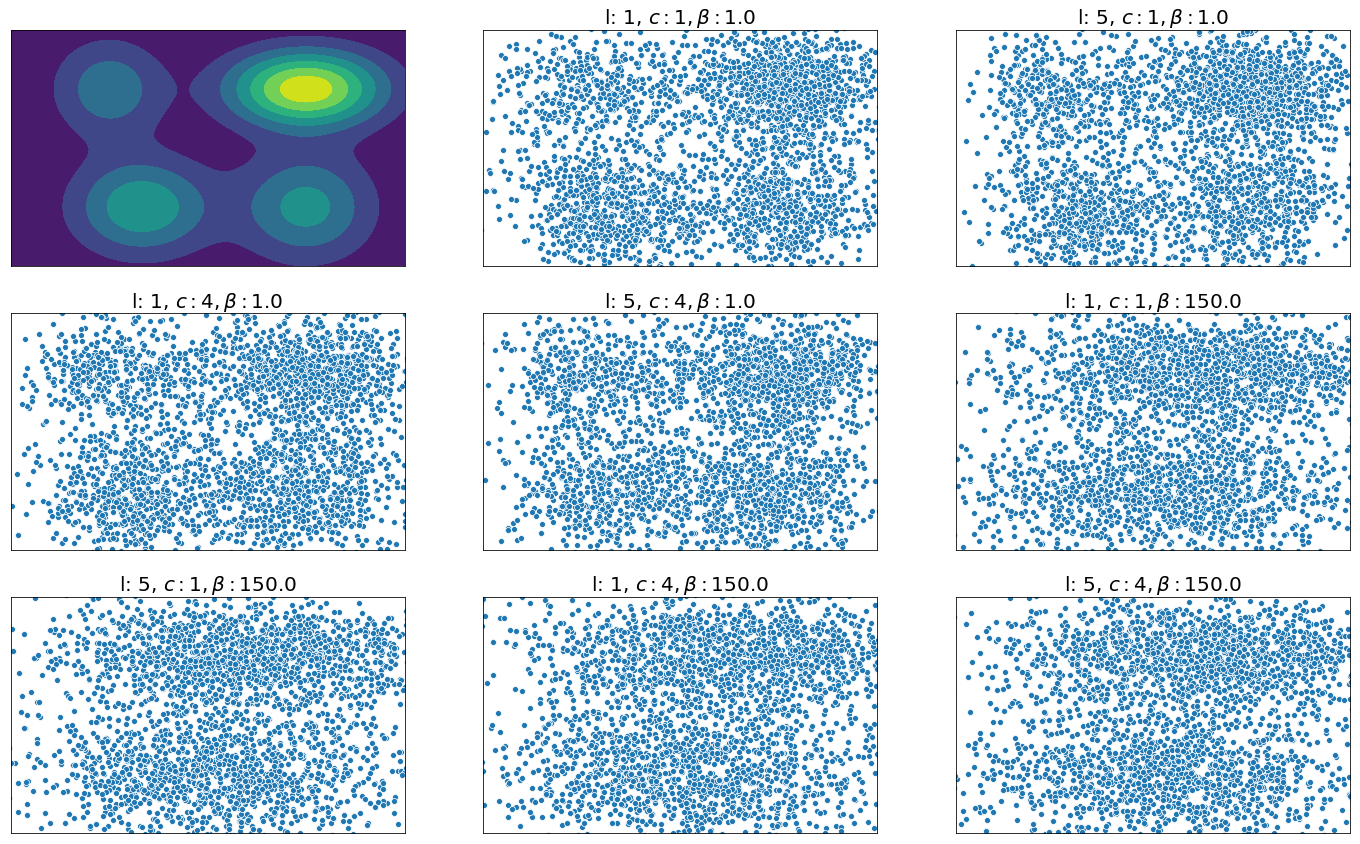
\includegraphics[width=0.8\linewidth]{img/multimodal_bivariate}
\caption{The top left image shows the contour plot of the multimodal mixture distribution. The remaining plots show samples from the decoder using different latent sizes, number of components and changing $\beta$ parameter.}
\label{fig_multimodal_bivariate}
\end{center}
\end{figure}

\fi

\section{The MuJoCo simulator and scenarios}

MuJoCo \parencite{todorov2012mujoco}, short for Multi-Joint dynamics with Contact, is a physics engine, suited in particular for simulating complex dynamic systems in contact-rich scenarios. Performance on robotics-like scenarios simulated by MuJoCo is now frequently reported when analyzing performance of RL algorithms~\parencite{duan2016benchmarking, popov2017data}.

For these experiments, we construct scenarios in MuJoCo and select parameters $\vec{\psi}$ that we wish to learn to reduce the reality gap. %We then observe the scenarios with a distribution over these parameters $\vec{\psi}$. 

In this context, \textit{real} data refers to trajectories generated via the simulator with a known configuration of the parameters with slight Gaussian noise. This noise is introduced during simulation and not added to observations. While this does not guarantee that \dettostoc{} works on actual real-world data, there are other benefits to conducting the experiments this way. One positive bonus with synthesizing \emph{real} data is that we can generate a variety of different physics dynamics to represent different versions of reality and make sure that the algorithm can find the correct set of parameters that best represent that particular system. Moreover, a plethora of test data can be generated to verify the quality of the results.

\subsection{Parameters and their meanings}
In the following experiments when we refer to friction we mean isotropic tangential friction between two geoms in MuJoCo. In MuJoCo, wind is a vector that is subtracted from the 3D translational velocity of each body, and the result is used to compute viscous, lift and drag forces acting on the body in passive dynamics. In the Windy Slope scenario, wind is only used along one axis, perpendicular to the inclination of the slope and thus causes the box to move sideways. For more information about how MuJoCo computes friction, contact detection and other forces, please see the Computation part at: \url{mujoco.org/book/computation.html}.

\section{Windy Slope scenario}
\label{windyslope}

\begin{figure}
\begin{subfigure}{\textwidth}
  \centering
  \begin{overpic}[trim=800 100 800 300,clip,width=0.3\textwidth]{img/windyslope/traj/windyslope-real-0}
      \put(2,2) {\color{white}$t=0$}
  \end{overpic}
  \begin{overpic}[trim=800 100 800 300,clip,width=0.3\textwidth]{img/windyslope/traj/windyslope-real-all-obstacle-50}
      \put(2,2) {\color{white}$t=50$}
  \end{overpic}
  \begin{overpic}[trim=800 100 800 300,clip,width=0.3\textwidth]{img/windyslope/traj/windyslope-real-all-obstacle-100}
      \put(2,2) {\color{white}$t=100$}
  \end{overpic}
\end{subfigure}

\caption{The \ws{} scenario, where a box with hidden inner content is placed on a sloping surface exposed to wind. The figure shows the environment at different timesteps $t$, and the position and orientation of the box have been superimposed in each image to give a sense of the randomness over time. The trajectory depends on samples from the slightly noisy \textit{real} parameter distributions: $\pfriction \sim \N(0.23, 0.01^2)$, $\pcom \sim \N(0.11, 0.04^2)$ and $\pwind \sim \N(-1.7, 0.05^2)$. The choice of means were picked at random, and the variances were selected to be small yet slightly stochastic to resemble the unpredictability of the real world.}
\label{fig:windyslope_real}
\end{figure}

\begin{figure}
\begin{subfigure}{\linewidth}
    \centering
    \begin{overpic}[trim=800 100 800 300,clip,width=0.4\linewidth]{img/windyslope/traj/windyslope-fake-wind-50}
        \put(2,2) {\color{white}$t=50$}
    \end{overpic}
        \begin{overpic}[trim=800 100 800 300,clip,width=0.4\linewidth]{img/windyslope/traj/windyslope-fake-wind-99}
        \put(2,2) {\color{white}$t=100$}
    \end{overpic}
    \caption{$\vec{\pwind} \sim \N(-1.0,0.5)$ with $\vec{\pfriction}$ and $\vec{\pcom}$ fixed.}
    \label{fig:traj_wind}
\end{subfigure}
\begin{subfigure}{\linewidth}
    \medskip
    \centering
    \begin{overpic}[trim=800 100 800 300,clip,width=0.4\linewidth]{img/windyslope/traj/windyslope-friction-50}
        \put(2,2) {\color{white}$t=50$}
    \end{overpic}
        \begin{overpic}[trim=800 100 800 300,clip,width=0.4\linewidth]{img/windyslope/traj/windyslope-friction-99}
        \put(2,2) {\color{white}$t=100$}
    \end{overpic}
    \caption{$\vec{\pfriction} \sim \N(0.25,0.1)$ with $\vec{\pwind}$ and $\vec{\pcom}$ fixed.}
    \label{fig:traj_friction}
\end{subfigure}
%
\begin{subfigure}{\linewidth}
    \medskip
    \centering
    \begin{overpic}[trim=800 100 800 300,clip,width=0.4\linewidth]{img/windyslope/traj/windyslope-fake-brick-i-1}
        \put(2,2) {\color{white}$t=0$}
    \end{overpic}
    \begin{overpic}[trim=800 100 800 300,clip,width=0.4\linewidth]{img/windyslope/traj/windyslope-fake-brick-i-50}
        \put(2,2) {\color{white}$t=50$}
    \end{overpic}
    \caption{Inner box placed at $\pcom=\{-0.45, 0, 0.45\}$.}% from left to right respectively.}
    \label{fig:traj_inner_box}
\end{subfigure}
%
\begin{subfigure}{\linewidth}
    \medskip
    \centering
    \begin{overpic}[trim=800 100 800 300,clip,width=0.4\linewidth]{img/windyslope/traj/windyslope-fake-all-50}
        \put(2,2) {\color{white}$t=50$}
    \end{overpic}
        \begin{overpic}[trim=800 100 800 300,clip,width=0.4\linewidth]{img/windyslope/traj/windyslope-fake-all-100}
        \put(2,2) {\color{white}$t=100$}
    \end{overpic}
    \caption{All three parameters sampled from initial estimate for $\vec{\psi}.$}
    \label{fig:traj_fake_all}
\end{subfigure}
\caption{Similar to Figure \ref{fig:windyslope_real}, this figure shows snapshots of the environment with parameters sampled from the initial simulation parameters $\vpsi$. To illustrate how each parameter affects the dynamics of the environment, (\subref{fig:traj_wind}) shows the impact of varying wind while keeping the other variables fixed. Similarly, (\subref{fig:traj_friction}) shows varying friction affects with the other variables kept fixed. (\subref{fig:traj_inner_box}) shows three boxes each with the inner box placed in different locations. In (\subref{fig:traj_fake_all}), all three parameters are sampled from $\vpsi$.}
\label{fig:windyslope_psi}
\end{figure}

A first scenario was constructed using MuJoCo in order to see if the \dettostoc{} algorithm can predict the next state given the current state while only simulating passive dynamics.

In this scenario, which can be seen in Figure \ref{fig:windyslope_real}, an object is placed on a sloping surface. To make the scenario more challenging and to emulate a situation where a parameter cannot be measured, another object is placed inside the box at an unknown position, thus altering the center of mass of the box. Furthermore, a fixed cylindrical obstacle placed in the middle of the surface, since accurately modelling contact is difficult and should make predicting the output slightly harder. 

How the box moves on the surface depends on the following variables: the tangential friction coefficients between the surface and the box, $\pfriction$, its center of mass, $\pcom$, as well as viscous, lift and drag forces caused by wind, $\pwind$. The goal is to predict the next state $\vns$ given current state $\vs$, with no knowledge of the \textit{real} variables for friction and wind. The state is an 18D vector consisting of the current position, orientation, linear and angular velocity of the object.

Following the \dettostoc{} algorithm outlined in \ref{det2stoc:algorithm}, we define initial distributions in parameter space $\vec{\psi}$ as wide truncated Gaussians. For this experiment, these initial estimates are purposely made uninformative as a proof of principle. For example, the prior distribution for $\pwind$ implies we do not know which way the wind is blowing. In reality however, the estimates can be based on observing the dynamics in the real world and trying to replicate the same behavior in the simulator.

The position and velocity of the object are recorded every 40ms during four seconds, corresponding to 100 timesteps. Each time the environment is reset, new parameters are sampled from $\vpsi$.

%During the first trial, to keep things less complex, we keep two of the variables fixed while strictly varying the third. This ensures that the particular variable can be identified without interference of the other two variables. The results can be seen in Figure \ref{fig_1_parameter}.

We vary all three parameters: \textit{friction, center of mass, wind}. How the environment changes with these parameters is illustrated in Figure \ref{fig:windyslope_psi}.

We run four iterations of \dettostoc{} and evaluate the log likelihood of the test set $\trajreal$ after each iteration. The results are presented in Table \ref{table:windyslope_results}, and visual plots showing the latent space encodings converging towards the \emph{real} parameters in Figure \ref{fig:windyslope_latent_space}.

%Then, using \textit{real} data, the \cvae{} is trained to output the next state given current state. We restrict the latent space to be equal to the number of variable parameters, in this case three: \textit{friction, impratio} and \textit{wind}.


%In theory, what is likely to happen is that the latent space captures the underlying parameters that would align simulations with the real world.
%To see if \dettostoc{} can generalize to more than one parameter, we simply choose an arbitrary value for another parameter and collect data in simulation on a range of reasonable values.

% \begin{figure}
%     \centering
%     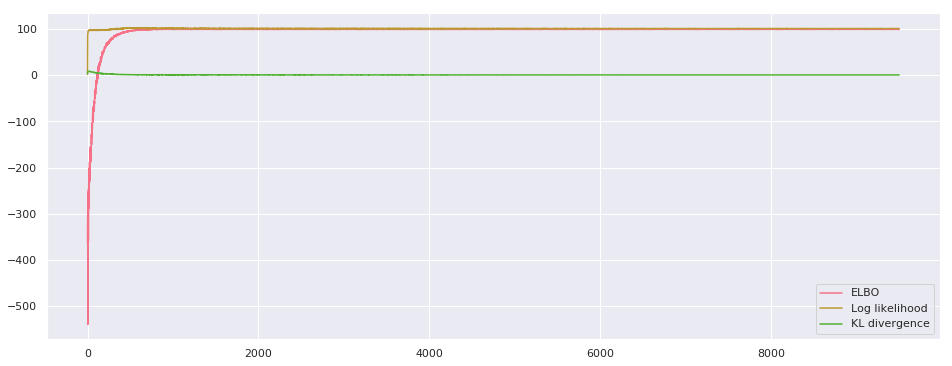
\includegraphics[width=\textwidth]{img/windyslope/windyslope_elbo.png}
%     \caption{ELBO plotted of validation set during training of ''real'' data $\vec{\xi}$}
%     \label{fig:my_label}
%     \todo[inline]{Will fix this plot.}
% \end{figure}

\begin{table}
\ra{1.3}
\centering

\begin{tabular}{lrr}
\multicolumn{3}{c}{\MakeLowercase{\textsc{\ws{} scenario}}} \\
\toprule
Model & \# Trajectories (samples) & Log likelihood  \\
\midrule
%\cvae{} (baseline) & 5 (500) & 22.09 \\

% delta 10 68.30329 71.555916 70.52932 70.049164 66.66855 72.10237
\cvae{} (baseline) & 10 (1000) & 69.42 $\pm$ 1.73\\

% 20: 85.45479
% 92.60568

\dettostoc{} (1 iter) & 10 (1000) & 69.26 $\pm$ 0.54 \\
\dettostoc{} (2 iter) & 10 (1000) & 73.72 $\pm$ 0.33 \\
\dettostoc{} (3 iter) & 10 (1000) & 76.36 $\pm$ 0.61 \\

% 74.901566 74.901566 79.11099
\dettostoc{} (4 iter) & 10 (1000) & \textbf{79.13 $\pm$ 0.11} \\

\bottomrule
\end{tabular}
\label{table:windyslope_results}
\bigskip

\caption{Log likelihood results test set on the \ws{} scenario. The baseline model has seen a total of 1000 \emph{real} samples. So has the \dettostoc{} model, however, it has also been trained on simulated data, parameterized by $\vpsi$ that we learned. We selected 1000 samples, or 10 trajectories, as a number that would be feasible to collect in the real world for most scenarios.}
\label{fig:windyslope_logprob}
\end{table}

We compare the results of \dettostoc{} against a \textbf{baseline} \cvae{} with the same number of layers and hidden units. This baseline \cvae{} is trained strictly on \emph{real} data and serves as an indication of the predictive performance without alignment with simulation data.
The log likelihood of the test set gives an indication of the quality of the predictions, but it is not very useful in order to understand how accurate the predictions are. It is obvious that the log likelihood of \dettostoc{} is better than a \cvae{} baseline that has only trained on the \emph{real} data. So to instead better understand how \dettostoc{} performs, we compare it to the true underlying dynamics of the system $p \given{\vns}{\vs}$. To do this, we initialize the physics simulator with a fixed state $\vs$, sample from the \emph{real} parameter distribution $\vth$ and simulate passive dynamics to generate $\vns$. This will give us a probability distribution over the next state $\vns$ that we can compare to the results $\ptheta \given{\vns}{\vs}$ of the \cvae{}. The results for the position and linear velocity can be seen in Figure \ref{fig:output_distribution_step50_posvel_dettostoc} and \ref{fig:output_distribution_step50_posvel_baseline}. The full state observation visualization can be found in Appendix \ref{appendix:a}.

\begin{figure}
\centering
\emph{\textsc{\MakeLowercase{\ws{} scenario}}}
\begin{subfigure}{\textwidth}
    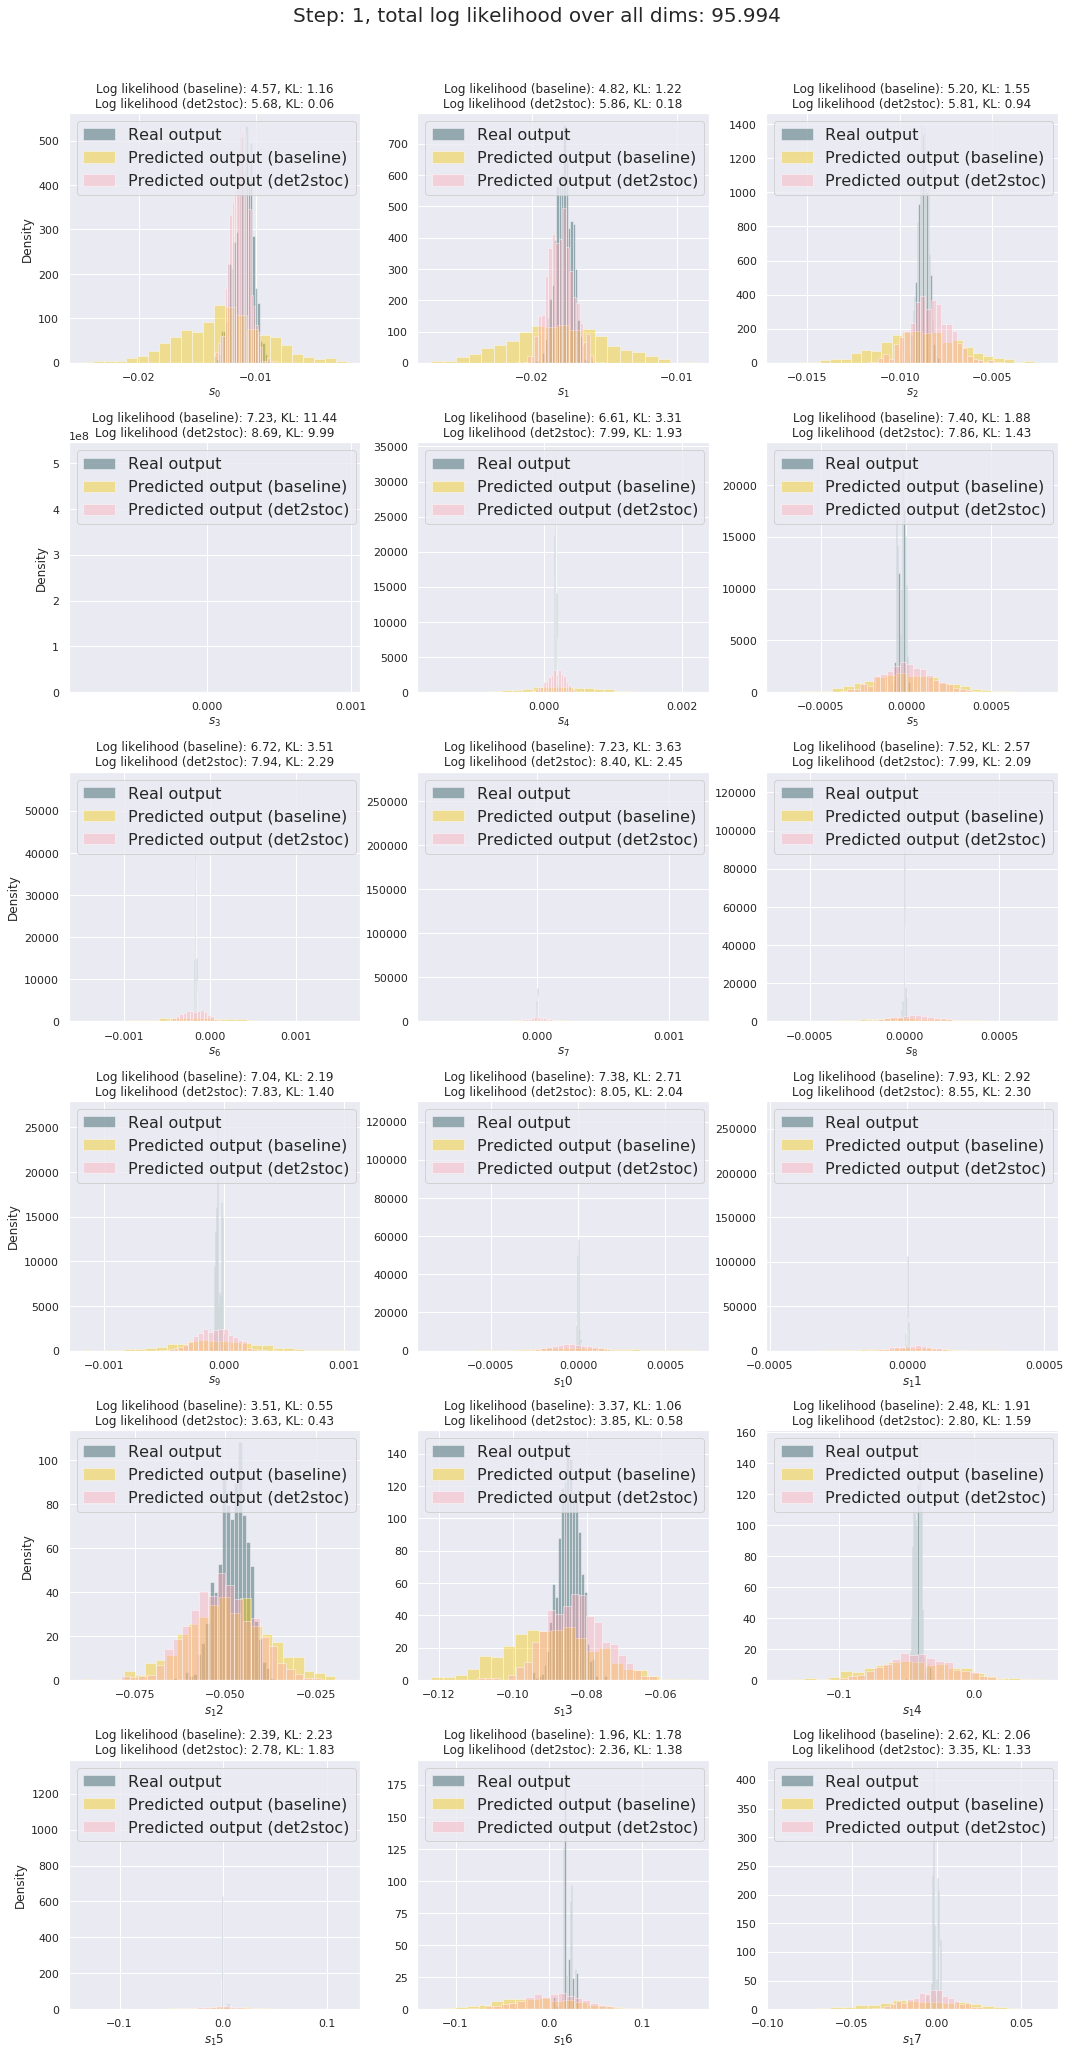
\includegraphics[trim=0 1650 0 50,clip,width=1.0\textwidth]
    {img/windyslope/output/output_distribution_step1_delta_all}
    \caption{$t=1$}
    \label{fig:output_distribution_step1_posvel_dettostoc}
\end{subfigure}
\begin{subfigure}{\textwidth}
    \centering
    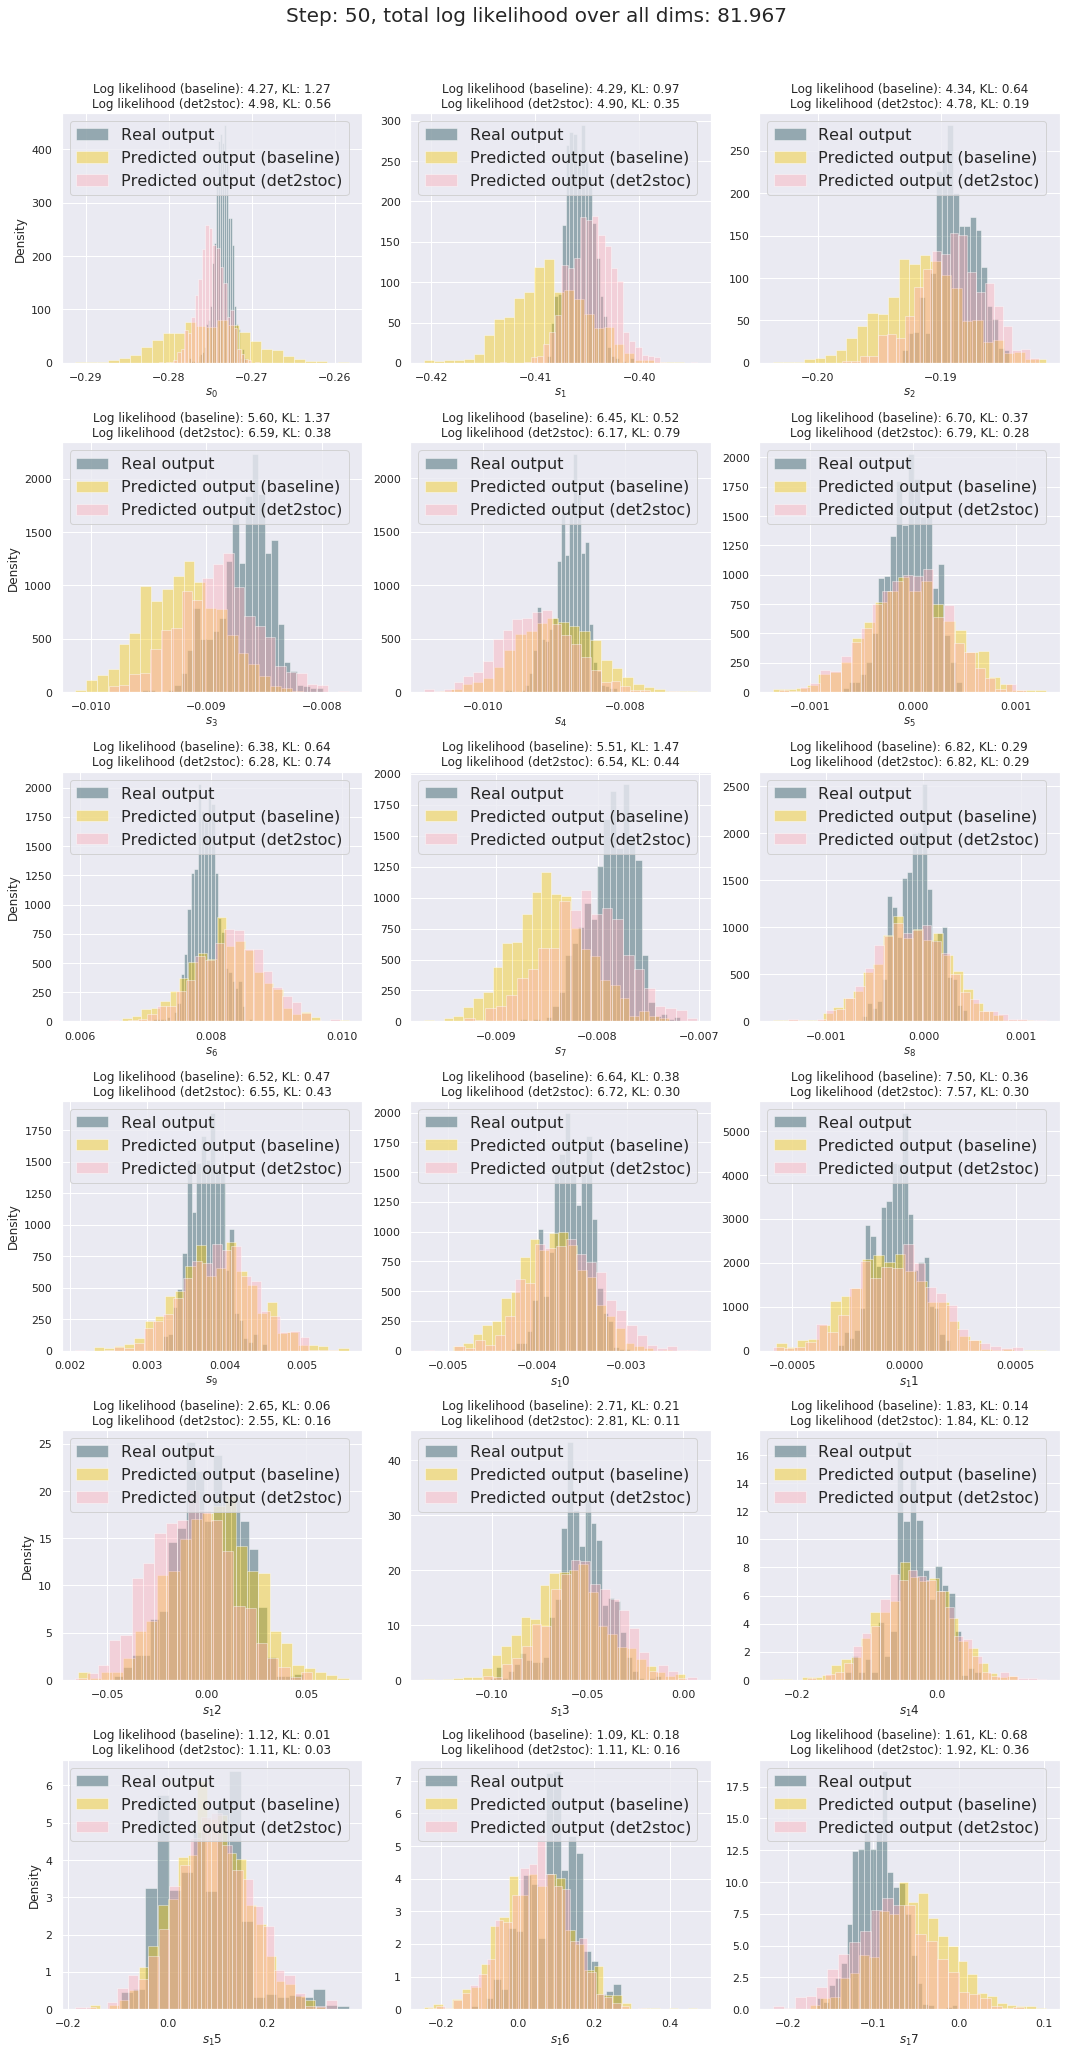
\includegraphics[trim=0 1650 0 50,clip,width=1.0\textwidth]
    {img/windyslope/output/output_distribution_step50_delta_all}
    \caption{$t=50$}
    \label{fig:output_distribution_step50_posvel_dettostoc}
\end{subfigure}
% \begin{subfigure}{\textwidth}
%     \centering
%     \includegraphics[trim=0 1650 0 50,clip,width=1.0\textwidth]
%     {img/windyslope/output/output_distribution_step100_delta_all}
%     \caption{$t=100$}
%     \label{fig:output_distribution_step100_posvel_dettostoc}
% \end{subfigure}
\caption{Prediction distributions $\ptheta \protect \given*{\vns}{\vs}$ over position outputs $(x,y,z)$ for a randomly sampled state at different timesteps $t$ for the simulator, the trained stochastic simulator trained with \dettostoc{} and the baseline. Above the plots are log likelihood of the \emph{real} output as well as sample KL divergence between the true distribution and the predicted distribution.
The full state output and additional timesteps can be found in Appendix \ref{appendix:a}.}
\end{figure}

\subsection{Retrieving parameter predictions using latent space codes}

As an experiment to see if \dettostoc{} can recover the \emph{real} parameters used by the simulator $\fsimulator_{\vth}$, we compute the expected mean and standard deviation of the posterior over the \emph{real} training set $\trajreal_{train}$. Since we have included the target $\vns$ in the posterior formulation, and pre-trained the decoder to match \fsimulator{}, samples from $\qphi \given{\vz}{\vs, \vns}$ should align with the true parameters $\vth$. The results can be seen in Table \ref{fig_3_parameters_table} and visually in Figure \ref{fig:windyslope_latent_space}.
%$\E_{\given{\vz}{\vs, \vns}}$

\begin{table}[h!]
\ra{1.3}
\centering
\begin{tabular}{lrrcrr}
\multicolumn{6}{c}{\textsc{windy slope scenario}} \\
\toprule
%& \multicolumn{2}{c}{\small\emph{Real}} & \phantom{a} & \multicolumn{2}{c}{\emph{Sim}} \\
%\cmidrule{2-3} \cmidrule{5-6}
& $\theta_\mu^{(true)}$ & $\phi_\mu^{(learned)}$ && $\theta_\sigma^{(true)}$ & $\phi_\sigma^{(learned)}$ \\
\midrule
% $\N$(0.25, 0.1) 
% $\N$(0, 0.2)
% $\N$(-1, 1.0) 

$\pfriction$ & 0.23 & 0.2308 && 0.01 & 0.0109 \\
$\pcom$ & 0.11 & 0.0985 && 0.04 & 0.0370 \\
$\pwind$ & -1.7 & -1.7075 && 0.05 & 0.0667 \\
\bottomrule
\end{tabular}
\caption{Latent representations of parameters $\vpsi$ in the windy slope scenario after running three iterations of \dettostoc{} starting from fairly uninformative priors for the parameters $\vpsi$. $\theta_\mu$ and $\theta_\sigma$ correspond to the mean and standard deviation of the \emph{real} parameters of the distribution, and $\phi_\mu$ and $\phi_\sigma$ correspond to the mean and standard deviation of samples from the posterior over the collected \emph{real} trajectories $\trajreal_{train}$. The initial prior and posterior parameters after each iteration of \dettostoc{} can be found in Appendix \ref{appendix:a}.}
\label{fig:windyslope_parameters_table}
\end{table}

\begin{figure}[h!]
\centering
\captionsetup{size=footnotesize}
\begin{subfigure}{\linewidth}
  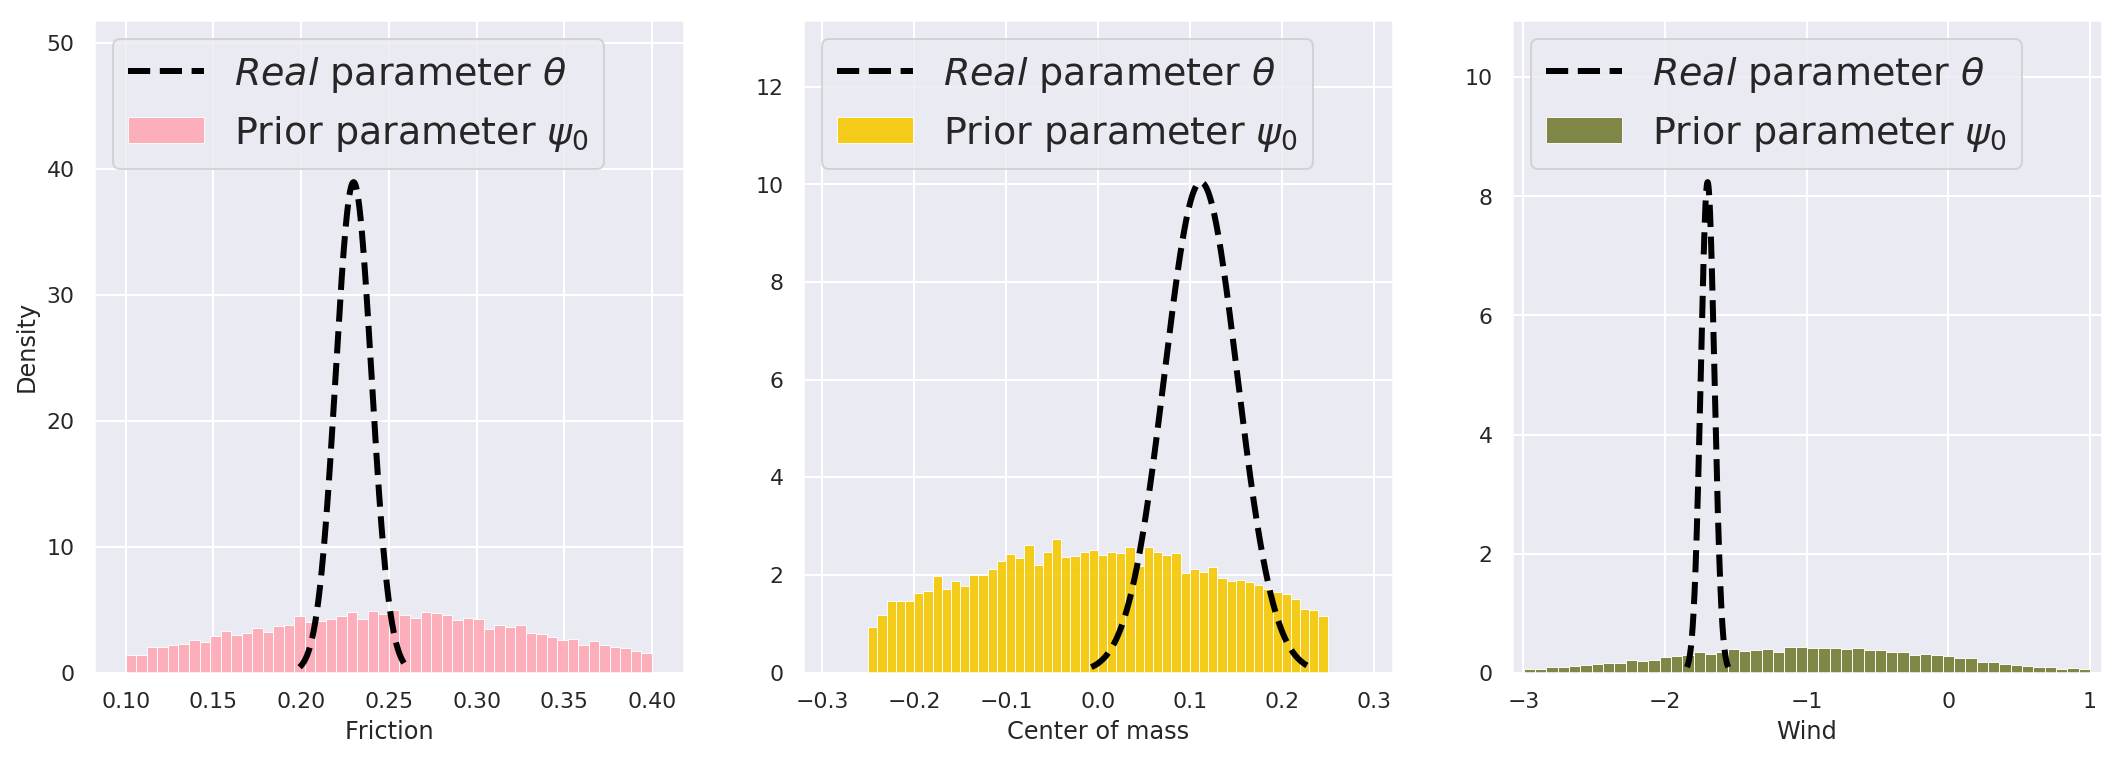
\includegraphics[width=1.0\linewidth]{img/windyslope/latent-representation/latent_encoding_iter0}
  \caption{$\vpsi_0$: initial estimates}
  \label{fig_3_parameters_0}
\end{subfigure}
\begin{subfigure}{\textwidth}
  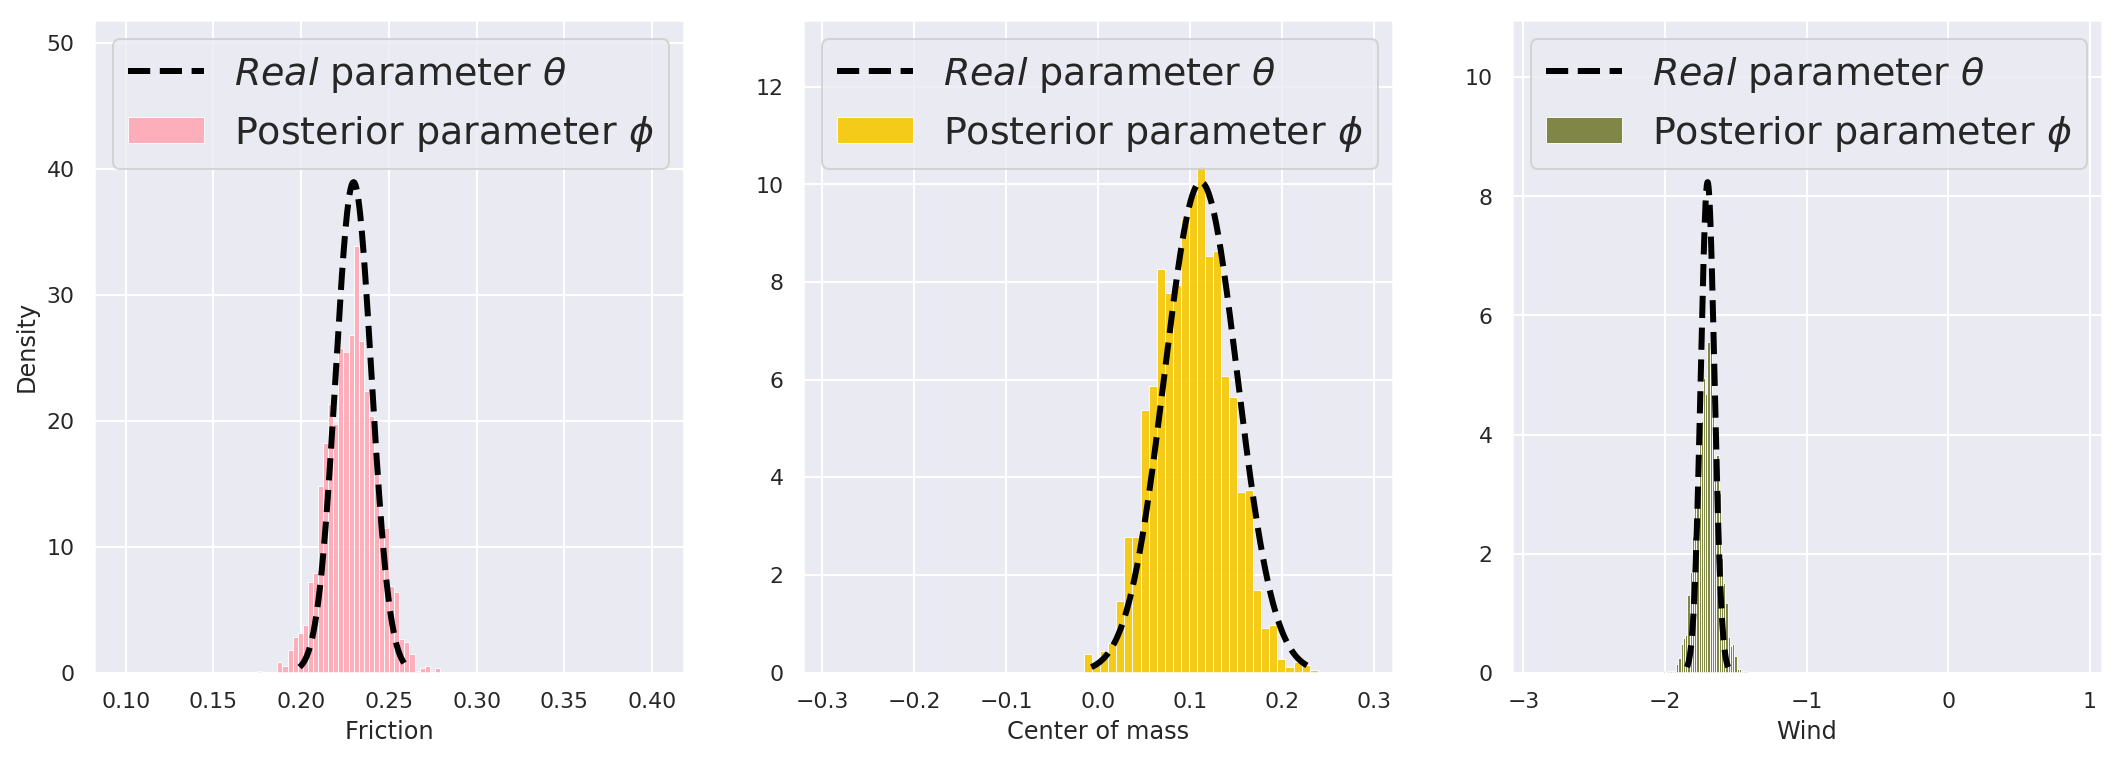
\includegraphics[width=1.0\linewidth]{img/windyslope/latent-representation/latent_encoding_iter3}
  \caption{$\vph3$ after 3rd iteration of \dettostoc{}}
\end{subfigure}
\caption{Plots show the learned parameters $\vph_{\mu, \sigma}$ of the posterior given \emph{real} samples $\vec{\xi}^{real}$ as normalized histograms after 3 iterations of \dettostoc{}.
From left-to-right, the latent space codings show tangential friction, center of mass and wind. %The prior parameters $\vpsi$ for each iteration of \dettostoc{} are included for clarity in a lighter color, along with the true distribution $\theta_{\mu, \sigma}$ in black dashes.}
The \emph{real} distribution of the parameters $\theta_{\mu, \sigma}$ in drawn with black dashes. Plots from previous iterations can be found in Figure \ref{fig:windyslope_latent_space_full} in Appendix \ref{appendix:a}.}
\label{fig:windyslope_latent_space}
\end{figure}

\clearpage
\section{\yp{} scenario}

A second scenario was constructed in MuJoCo that introduces control actions affecting the system dynamics. Similar to the Windy Slope scenario, a box with unknown center of mass is placed on a surface with unknown friction. However, inclination and wind have been removed and instead a robot interacts with the environment with the goal of pushing the box to a target goal.

The robot is an ABB IRB14000 YuMi with 2 arms, each with 7 joints corresponding to 14 degrees of freedom. The joints are actuated by velocity controllers. The real robot and the robot modelled in MuJoCo can be seen in Figure \ref{fig:robots}.

At the start of each episode, the arms are initialized to a default pose and the initial location of the box is placed randomly within a $0.2m \times 0.2m$ square area. The goal is kept fixed in the center of the table. The \emph{real} friction and center of mass distributions are listed in Table \ref{table:yumi_parameters}.

The goal is now to predict the next state $\vns$ given both $\vs$ and $\va$. The state consists of the position and velocity of all 14 joints, the position and orientations of the end effectors, as well as the position, rotation and velocity of the box.

The results can be found in Table \ref{table:yumi_results}. As the state vector is 60D we have chosen not to include the output distributions.

%The reward is a function of the distance: it is 0 outside a 0.14m radius of the goal, and otherwise monotonically increasing until the box is within 0.07m of the goal, which yields a reward of 1.


\begin{figure}%
    \centering
    \begin{subfigure}{0.4\textwidth}
    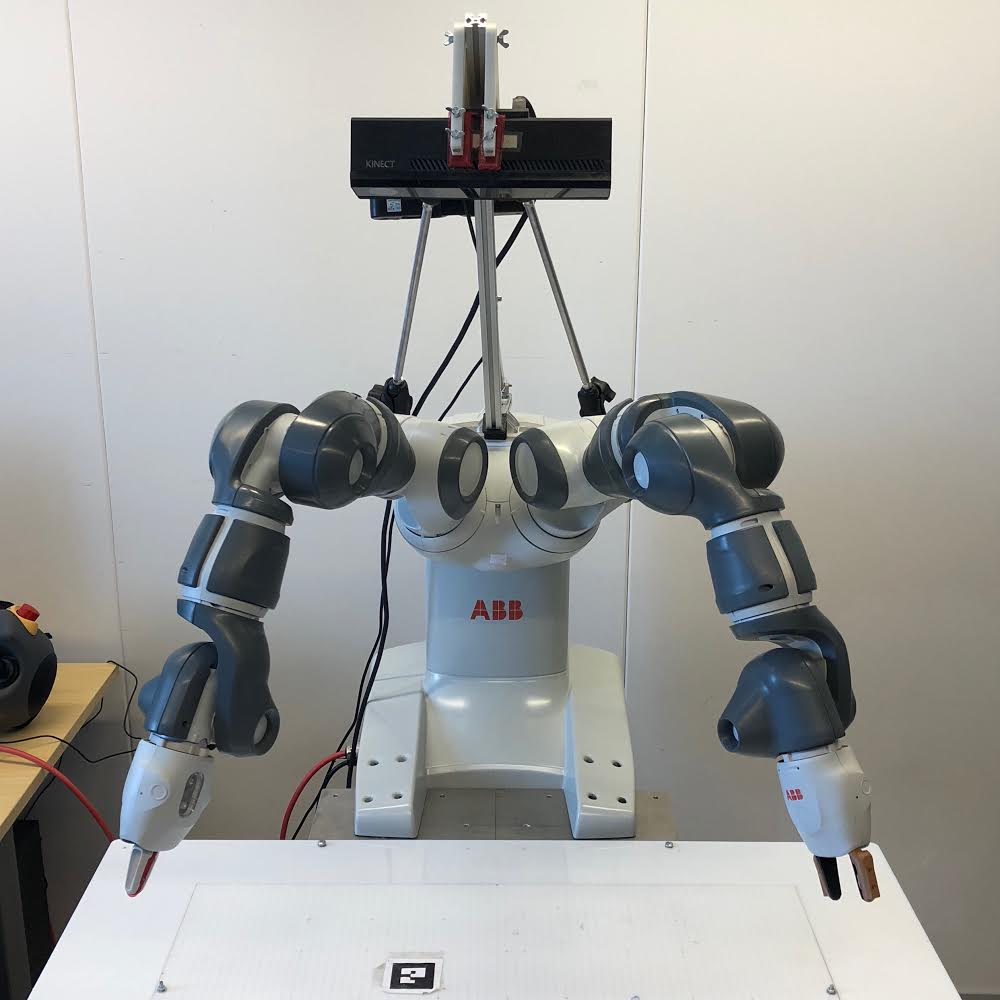
\includegraphics[width=1\textwidth,trim=0 0 0 0,clip]{img/yumi/yumi-pose-real}
    \end{subfigure}
    % \begin{subfigure}{0.4\textwidth}
    % 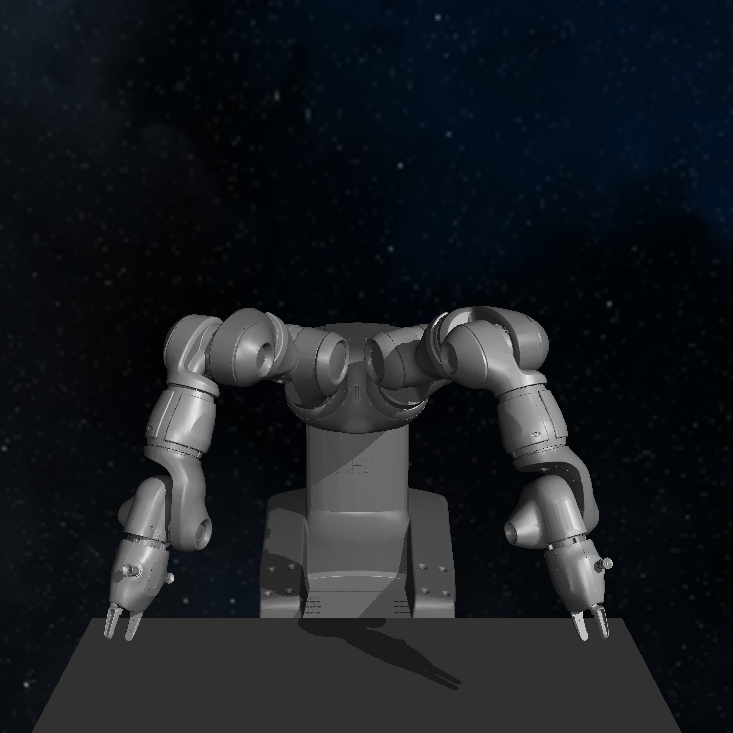
\includegraphics[width=1\textwidth]{img/yumi/yumi-pose-sim}
    % \end{subfigure}
    \begin{subfigure}{0.4\textwidth}
    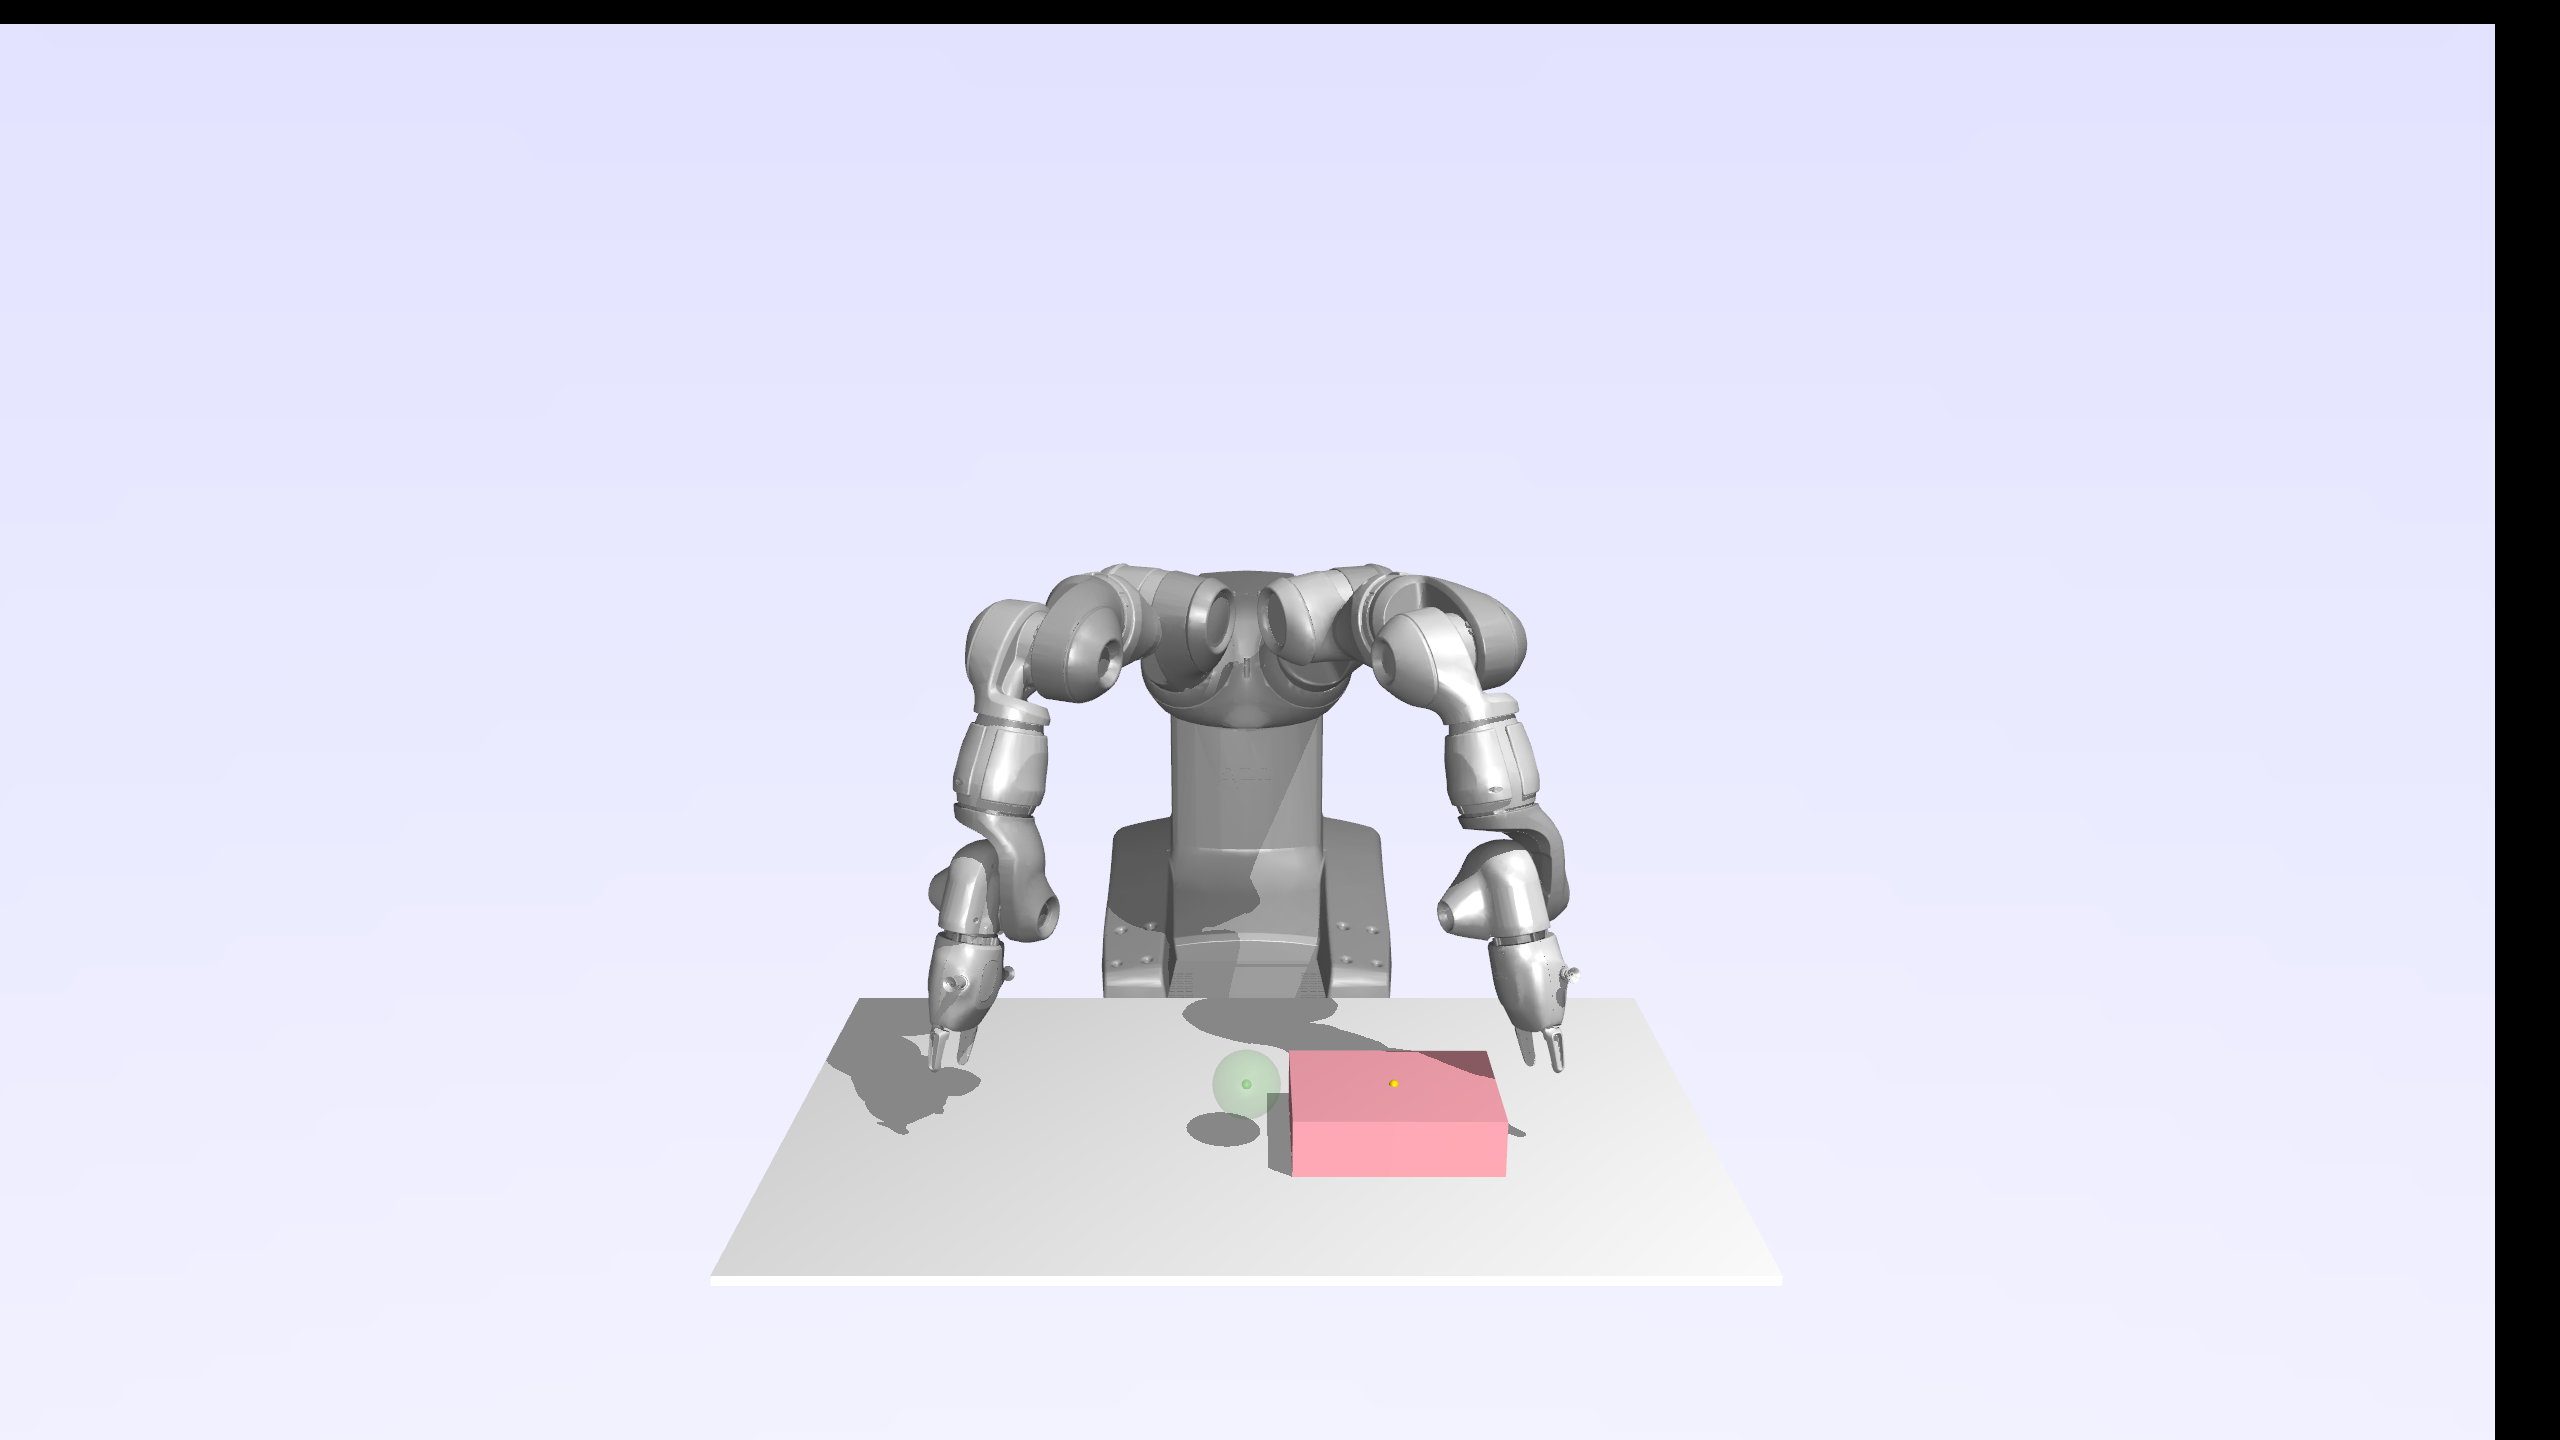
\includegraphics[width=1\textwidth,trim=800 240 810 250,clip]{img/yumi/yumi-pose-sim2}
    \end{subfigure}
    \caption{(Left) The real ABB YuMi IRB14000 robot. (Right) The robot modelled in MuJoCo for the box pushing scenario. The environment is considered complete when the yellow dot on the box is within the green sphere in the middle of the table.}
    \label{fig:robots}%
\end{figure}

\begin{table}
\ra{1.3}
\centering
\begin{tabular}{lrrcrr}
\multicolumn{6}{c}{\textsc{\MakeLowercase{\yp{} scenario}}} \\
\toprule
%& \multicolumn{2}{c}{\small\emph{Real}} & \phantom{a} & \multicolumn{2}{c}{\emph{Sim}} \\
%\cmidrule{2-3} \cmidrule{5-6}
& $\theta_\mu^{(true)}$ & $\phi_\mu^{(learned)}$ && $\theta_\sigma^{(true)}$ & $\phi_\sigma^{(learned)}$ \\
\midrule
$\pfriction$ & $0.28$ & $0.3404$ && $0.01$ & $0.1093$ \\
$\pcom$ & $0.035$ & $ 0.0367$ && $0.005$ & $0.0048$ \\
\bottomrule
\end{tabular}
\caption{Latent representations of parameters $\psi$ in the \yp{} scenario after running two iterations of \dettostoc{} starting from uninformed priors for the parameters $\vec{\psi}$. $\theta_\mu$ and $\theta_\sigma$ correspond to the mean and standard deviation of the \emph{real} parameters of the distribution, and $\phi_\mu$ and $\phi_\sigma$ correspond to the mean and standard deviation of samples from the posterior over the collected \emph{real} trajectories $\vec{\xi}^{real}$. \todo[inline]{These numbers will be updated with better results}}
\label{table:yumi_parameters}
\end{table}


\begin{table}
\ra{1.3}
\centering
\begin{tabular}{lrr}
\multicolumn{3}{c}{\textsc{\MakeLowercase{\yp{} scenario}}} \\
\toprule
%& \multicolumn{2}{c}{\small\emph{Real}} & \phantom{a} & \multicolumn{2}{c}{\emph{Sim}} \\
%\cmidrule{2-3} \cmidrule{5-6}
Model & \# \emph{Real} trajectories (samples) & Log likelihood over $\trajreal_{test}$ \\
\midrule
\cvae{} (baseline) & 10 (1000) & 306.4443\\
\cvae{} (baseline) & 900 (90000) & 680.5626 \\
\dettostoc{} (1 iter) & 10 (1000) & 673.4169\\
\dettostoc{} (2 iter) & 10 (1000) & 673.9966\\
\dettostoc{} (3 iter) & 10 (1000) & 706.21295\\
\dettostoc{} (4 iter) & 10 (1000) & \textbf{724.1508}\\

\bottomrule
\end{tabular}
\caption{Log likelihood results over the test set on the YuMi Box Pushing Scenario. \dettostoc{} has only seen 1000 \emph{real} samples but still outperforms the baseline model that has trained on 90000 samples.}
\label{table:yumi_results}
\end{table}


\begin{figure}
\centering
\captionsetup{size=footnotesize}
\begin{subfigure}{\textwidth}
  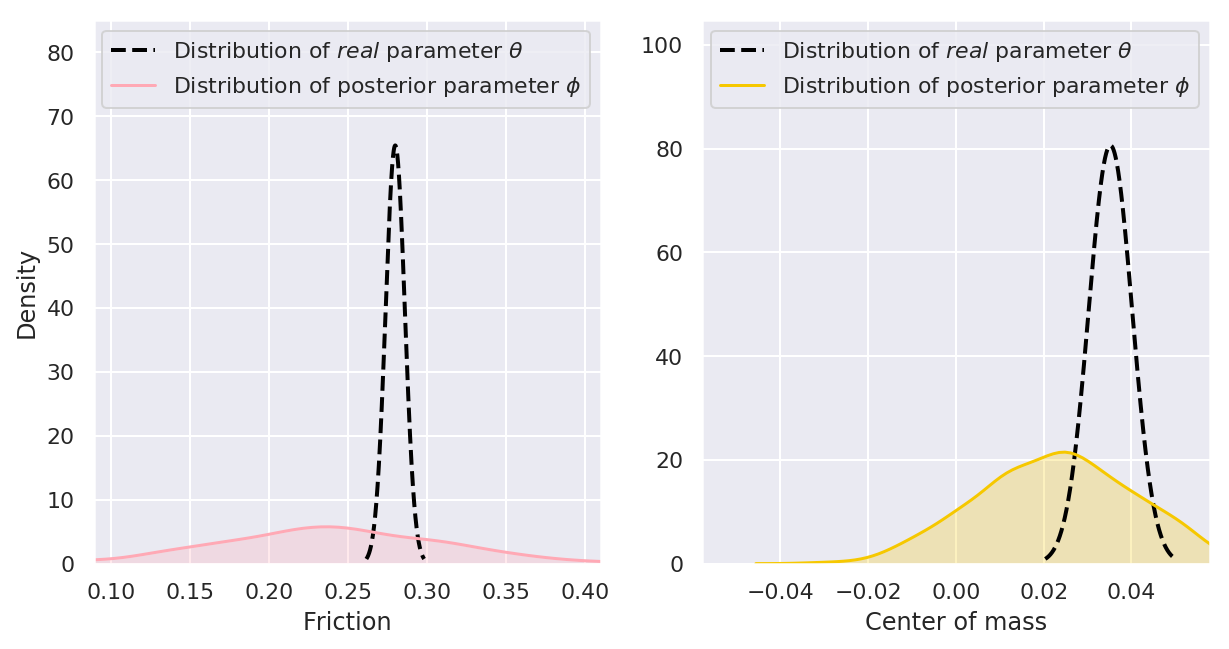
\includegraphics[width=\textwidth]{img/yumi/latent-representation/yumi_latent_encoding_0_iter}%
  \caption{Initial estimates of $\vpsi$ before \dettostoc{}}
\end{subfigure}
\begin{subfigure}{\textwidth}
  \centering
  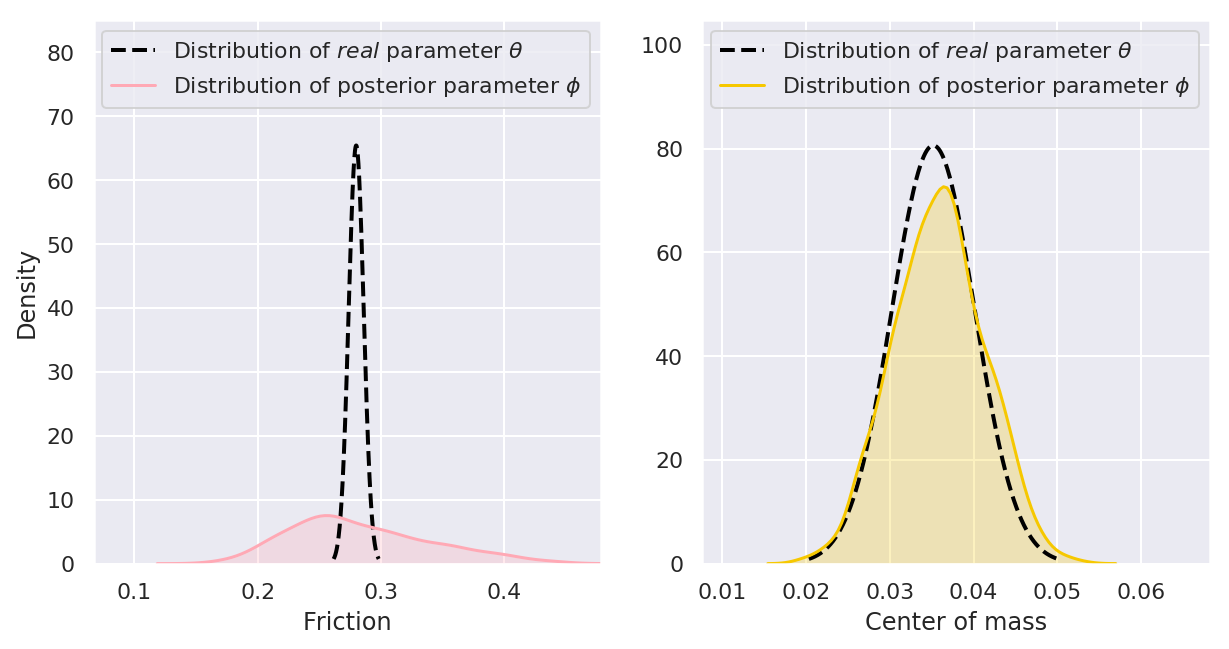
\includegraphics[width=\linewidth]{img/yumi/latent-representation/yumi_latent_encoding_3_iter}
  \caption{3rd iteration of \dettostoc{}}
\end{subfigure}
\caption{Plots show the learned parameters $\vph_{\mu, \sigma}$ of the posterior given \emph{real} samples $\vec{\xi}^{real}$ for the \yp{} scenario for four iteration of \dettostoc{}.
The parameters correspond (from left-to-right) to tangential friction $\pfriction$ and center of mass $\pcom$. The true distributions $\vth_{\mu, \sigma}$ are outlined in black dashes. In this scenario, \dettostoc{} struggles to match $\pfriction{}$ with the true distribution $\theta_\textsc{friction}$. This is likely due to the fact that the learned policy pushes the box in small increments, and small changes in friction do not cause any noticable difference. The posterior for all iterations can be found in the appendix.}
\label{fig:yumi_latent_space}
\end{figure}

\chapter{Conclusions}
\label{conclusions}

\section{Summary}

The proposed method in this thesis is built on the basis of the \vae{} and its conditionally modified variant \cvae{}. The \cvae{} was used to learn latent representations that can be used to ameliorate Sim-To-Real transfer by more accurately modelling reality in a data-efficient way. We incorporated the various techniques to avoid latent variable collapse. A baseline \cvae{} was trained on real data and required at least three times as many samples to be on par with \dettostoc{}.

The \dettostoc{} algorithm was tested on two MuJoCo scenarios. The two scenarios were similar, but the first scenario only simulated passive dynamics while the second one included a robot interacting with the system with control actions. In both scenarios, the \dettostoc{} exceedingly outperformed the baseline and correctly identified the distribution of the selected parameters to almost identical means and variances. On average, training a \cvae{} from scratch required four times as much data to achieve the same log likelihood of the real data.

We showed that the \dettostoc{} algorithm can be used as a data-efficient way to represent probability dynamics of robots and their environments.

\section{Discussion}

From the results, it is clear that \dettostoc{} can locate the mean but slightly underestimates the variance of parameters. This is a general problem of variational inference \parencite{bishop:2006:PRML} and not specific to the proposed methods.

\subsection{Constrained optimization}

The \dettostoc{} algorithm that has been outlined in this thesis does not enforce validness of the output. The loss used to optimize the predictions is the euclidean norm together with a divergence term. This means that no measures have been taken to ensure that the properties of the predicted output are valid. For example, if the output is a rotation matrix, it is not guaranteed to be orthogonal. However, this is not a limitation of the proposed \dettostoc{} algorithm, but rather a general problem when training neural networks. Moreover, this does not have any significant impact for the uses described in this thesis, but should be considered if the output is used in other systems that require correctness. %Different measures can be taken to avoid this problem. For example, if the rotation matrix $M$ needs to be orthogonal: let $M=U \Sigma V$ be the singular value decomposition of $M$, then $R=UV$.

\subsection{Future work}

For the experiments, we assume that the \textit{real} parameters lie in the interval of a prior guess. Future research should look into whether \dettostoc{} can indicate that the prior is outside the interval, and how well it handles more uninformed priors for the parameters.

Some work was done trying out a mixture of distributions as prior \parencite{DBLP:journals/corr/DilokthanakulMG16} but we found this approach ineffective in our experiments. \todo{Is Kingma's M2 model use a mixture as prior?}

We used a \cvae{} as a generative model. However, \dettostoc{} could be used with other generative models, such as Generative Adversarial Networks (GANs) \parencite{goodfellow2014} with some modifications.

We would like to extend our framework to real data and real robots in future work. Furthermore, we would incorporate higher-dimensional sensor modalities, such as vision, for both state observations and parameters of simulation randomization.

\todo{Importance weighted sampling from posterior} 

%======================================================
\printbibliography[heading=bibintoc]

\appendix
%======================================================
\label{appendix:a}

\begin{figure}
\centering
\text{Latent space encodings for the \textsc{Windy Slope Scenario}.}
\captionsetup{size=footnotesize}
\begin{subfigure}{\linewidth}
  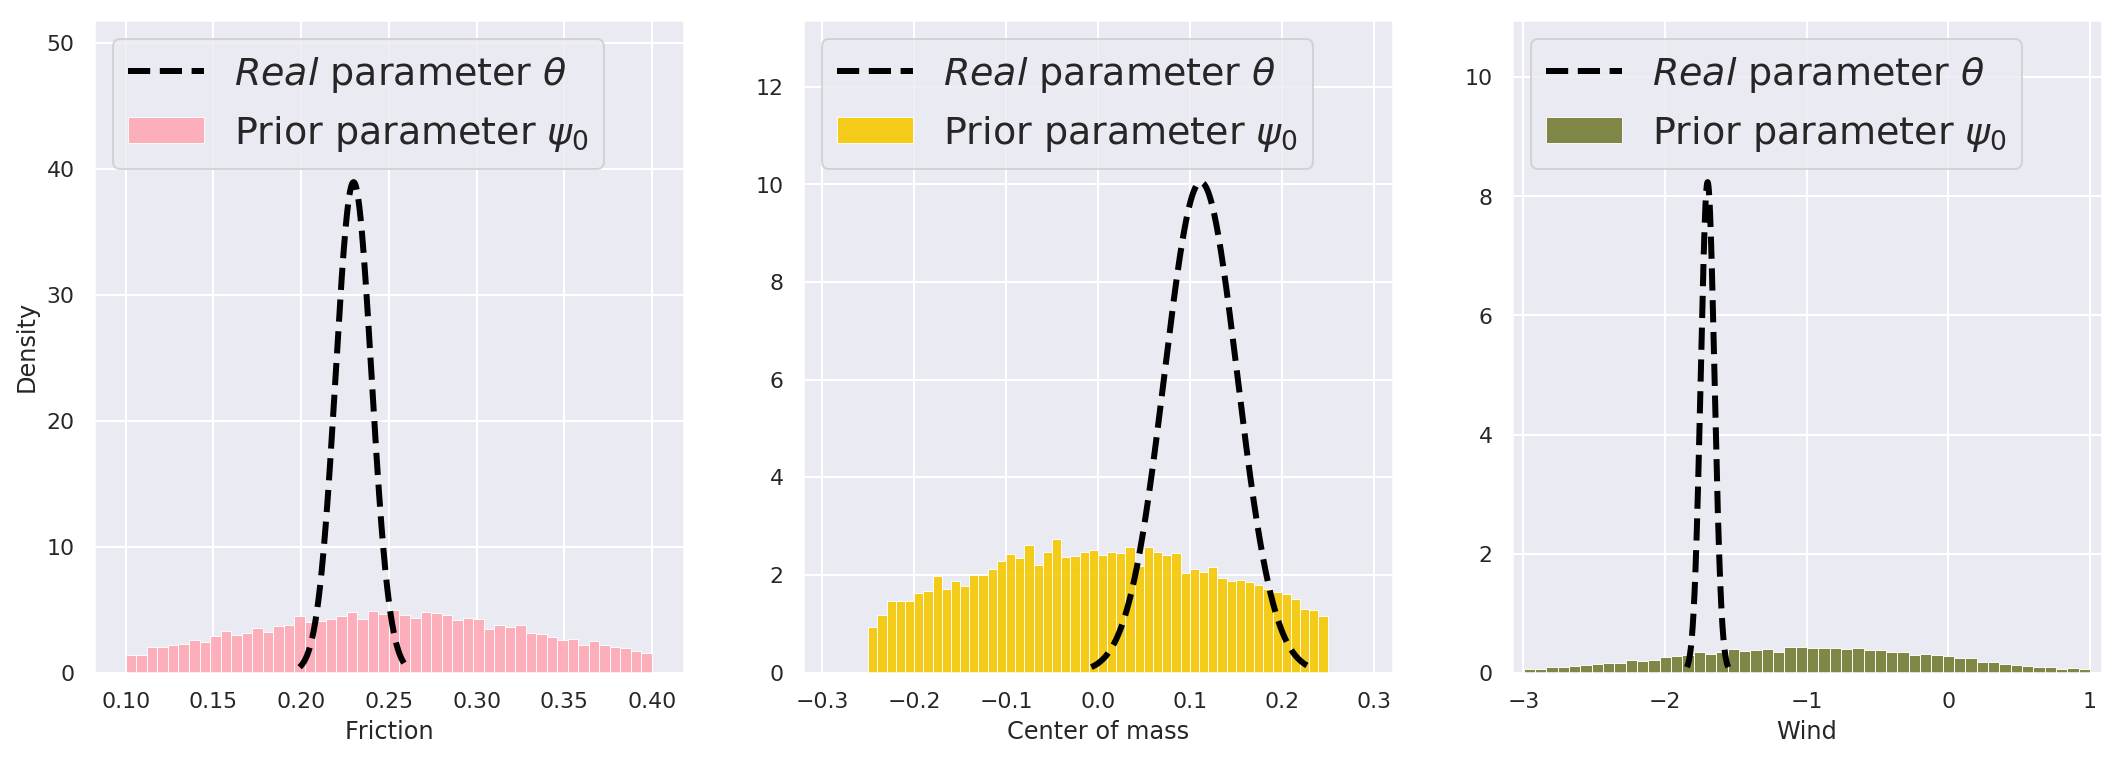
\includegraphics[width=1.0\linewidth]{img/windyslope/latent-representation/latent_encoding_iter0}
  \caption{Initial estimates of $\psi$}
  \label{fig_3_parameters_0}
\end{subfigure}
\begin{subfigure}{\linewidth}
  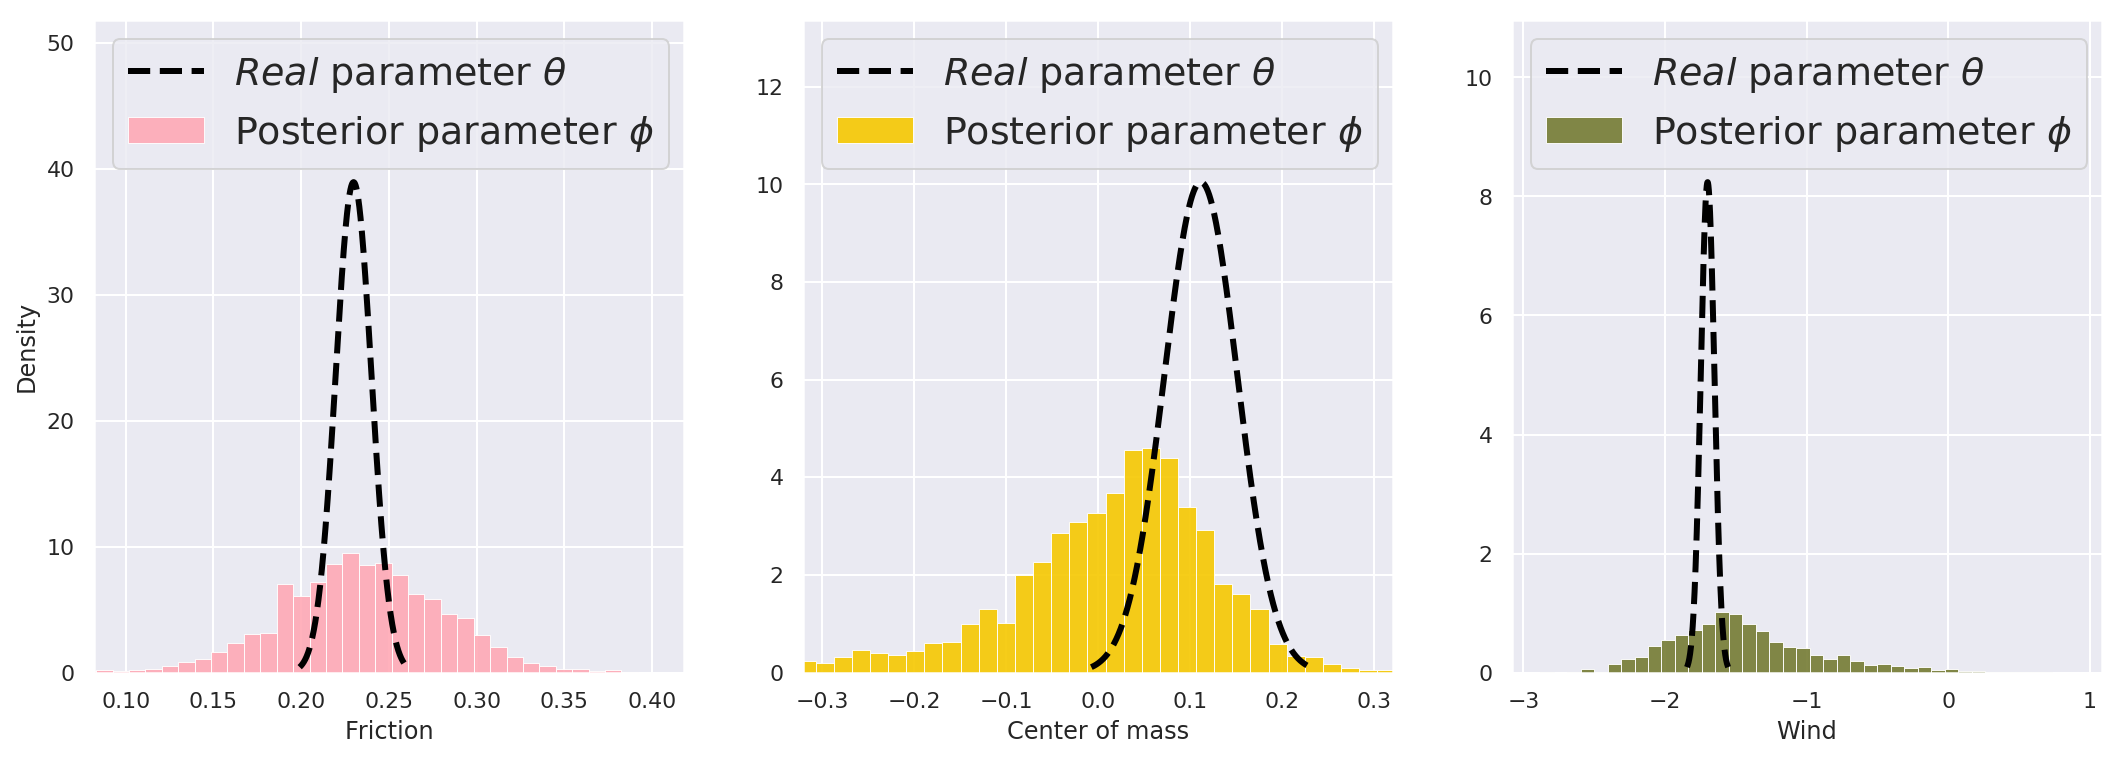
\includegraphics[width=1.0\linewidth]{img/windyslope/latent-representation/latent_encoding_iter1}
  \caption{1st iteration of \dettostoc{}}
  \label{fig_3_parameters_0}
\end{subfigure}
\begin{subfigure}{\textwidth}
  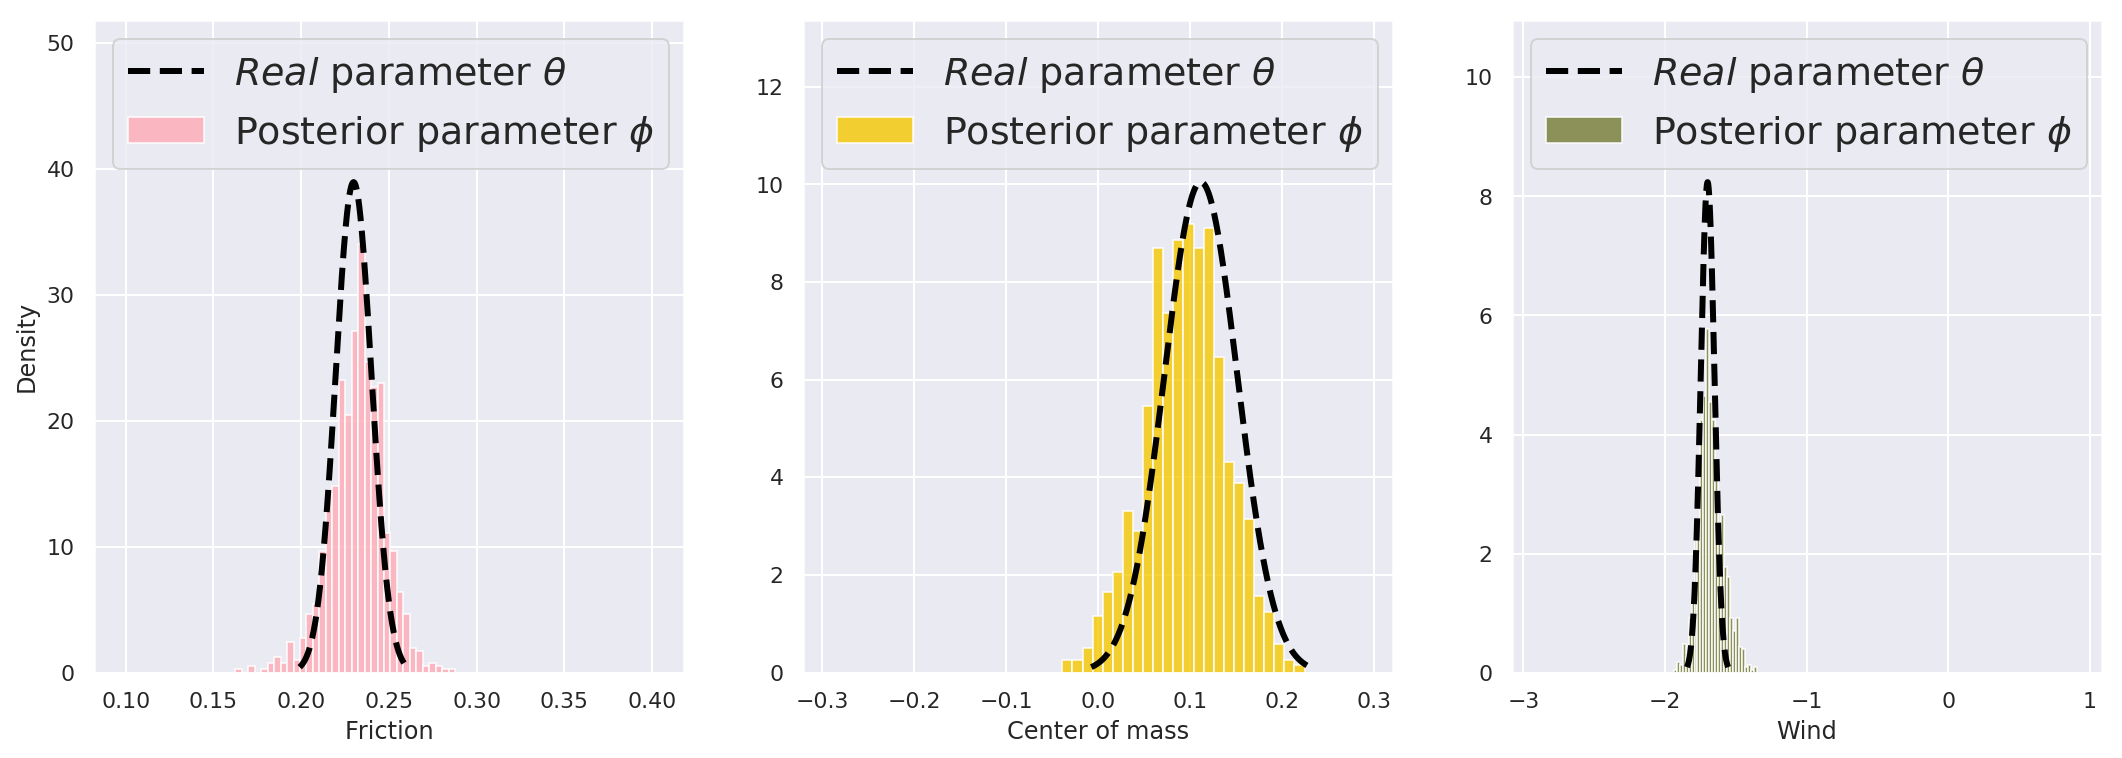
\includegraphics[width=1.0\linewidth]{img/windyslope/latent-representation/latent_encoding_iter2}
  \caption{2nd iteration of \dettostoc{}}
\end{subfigure}
\begin{subfigure}{\textwidth}
  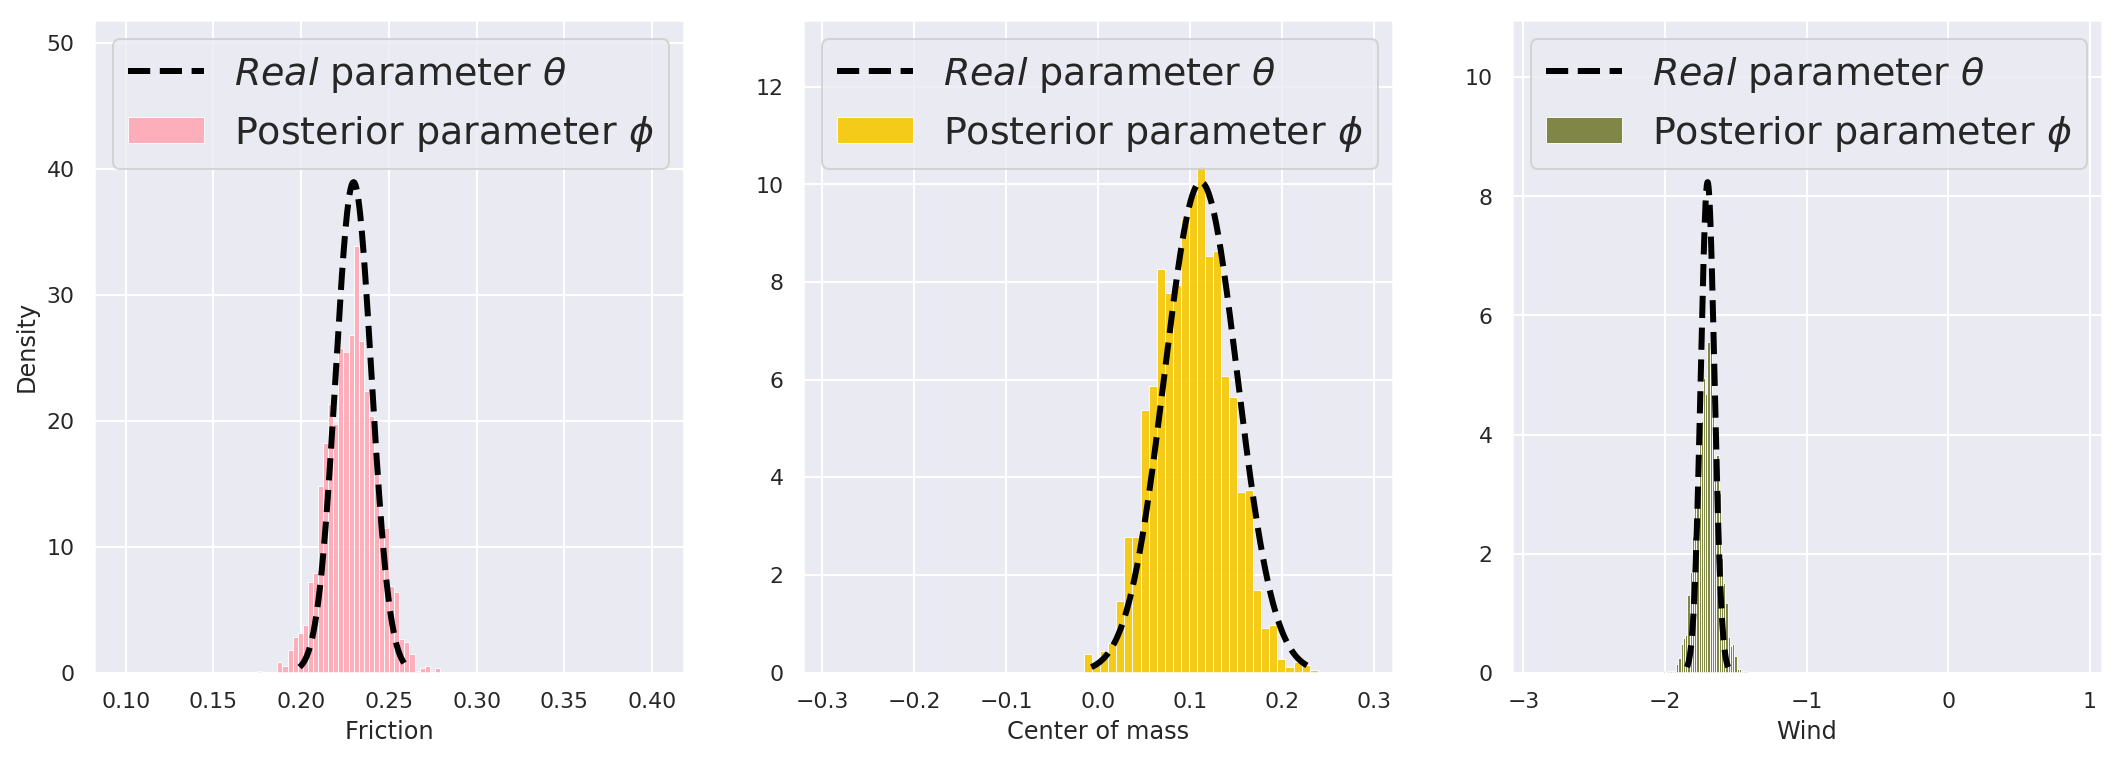
\includegraphics[width=1.0\linewidth]{img/windyslope/latent-representation/latent_encoding_iter3}
  \caption{3rd iteration of \dettostoc{}}
\end{subfigure}
\caption{Plots show the learned parameters $\vph_{\mu, \sigma}$ of the posterior given \emph{real} samples $\vec{\xi}^{real}$ as normalized histograms after subsequent steps of \dettostoc{}.
From left-to-right, the latent space codings show tangential friction, center of mass and wind. %The prior parameters $\vpsi$ for each iteration of \dettostoc{} are included for clarity in a lighter color, along with the true distribution $\theta_{\mu, \sigma}$ in black dashes.}
The \emph{real} distribution of the parameters $\theta_{\mu, \sigma}$ in drawn with black dashes.}
\label{fig:windyslope_latent_space_full}
\end{figure}

\begin{figure}
\centering
\text{Latent space encodings for the YuMi Box Pushing Scenario.}
\captionsetup{size=footnotesize}
\begin{subfigure}{0.45\textwidth}
  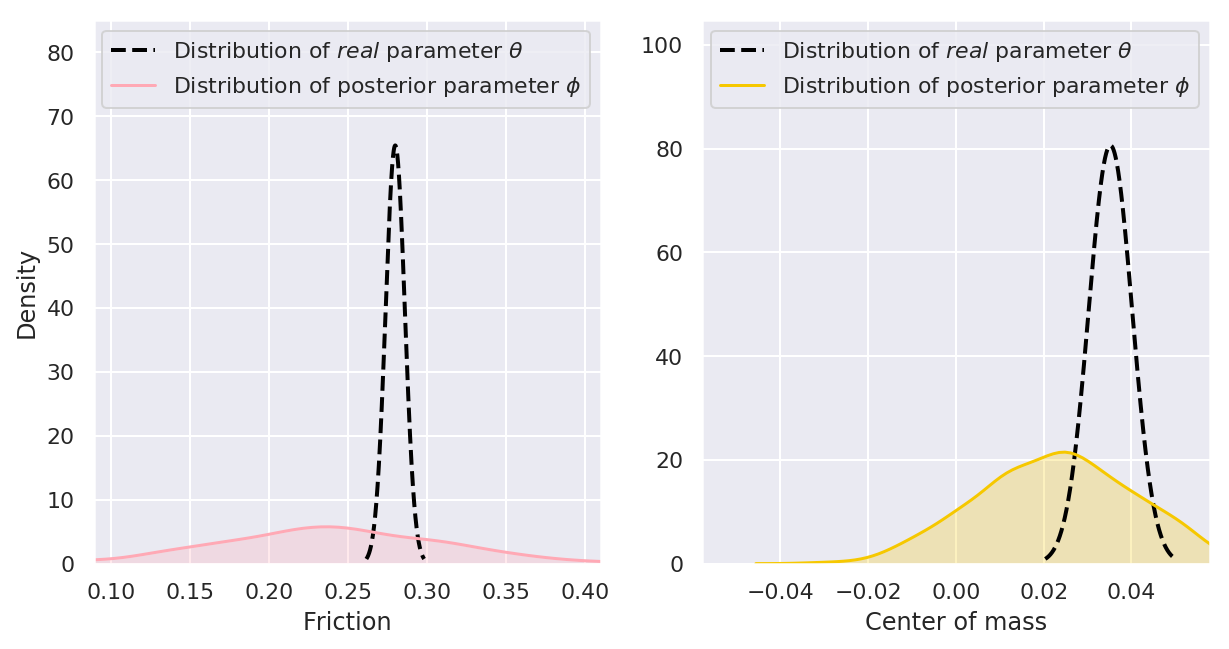
\includegraphics[width=\textwidth]{img/yumi/latent-representation/yumi_latent_encoding_0_iter}%
  \caption{Initial estimates of $\vpsi$ before \dettostoc{}}
\end{subfigure}
\begin{subfigure}{0.45\textwidth}
  \centering
  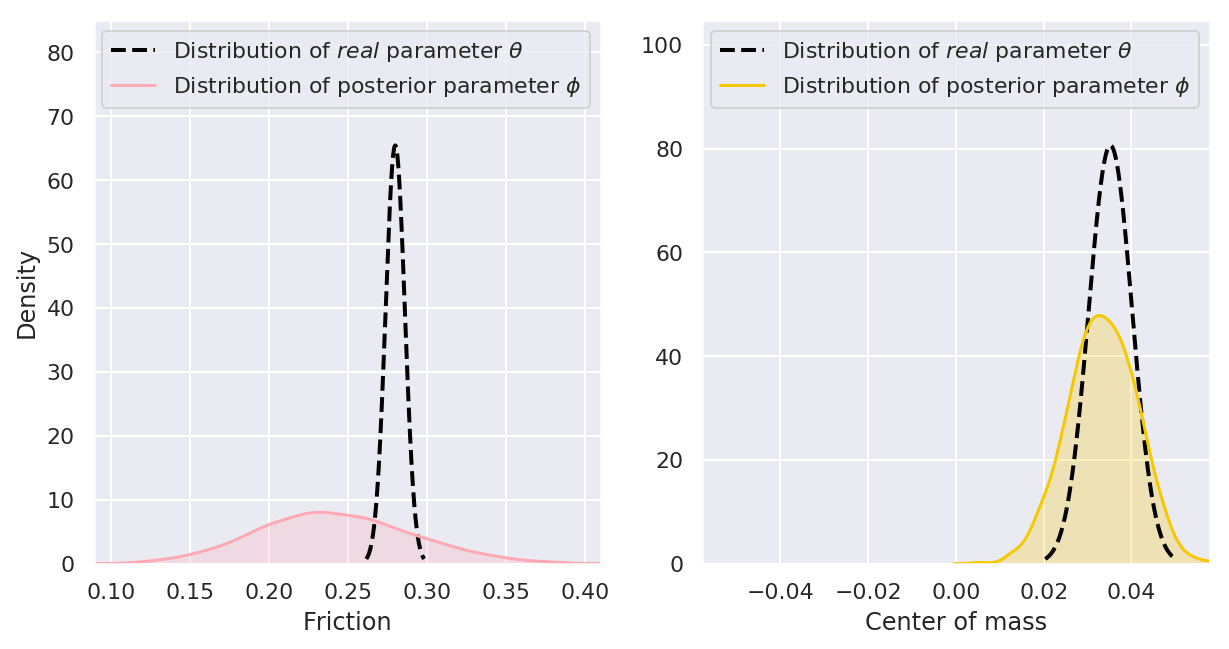
\includegraphics[width=\linewidth]{img/yumi/latent-representation/yumi_latent_encoding_1_iter}
  \caption{$\psi$ after 1st iteration of \dettostoc{}}
\end{subfigure}
\begin{subfigure}{0.45\textwidth}
  \centering
  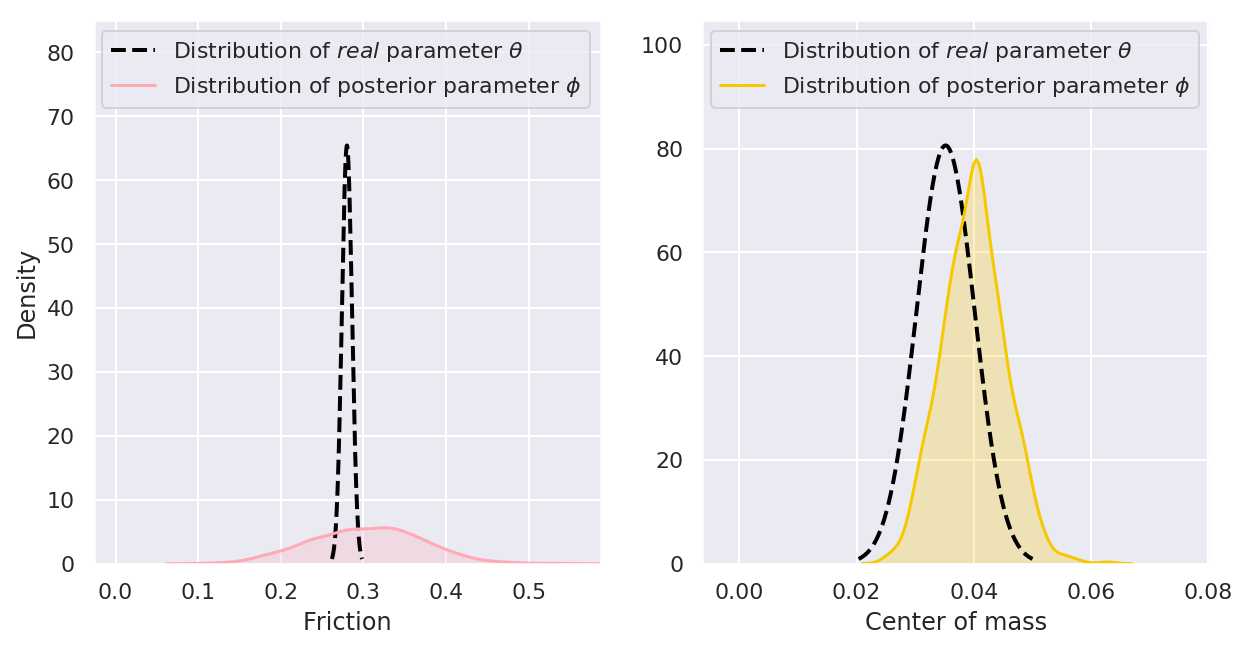
\includegraphics[width=\linewidth]{img/yumi/latent-representation/yumi_latent_encoding_2_iter}
  \caption{$\psi$ after 2nd iteration of \dettostoc{}}
\end{subfigure}
\begin{subfigure}{0.45\textwidth}
  \centering
  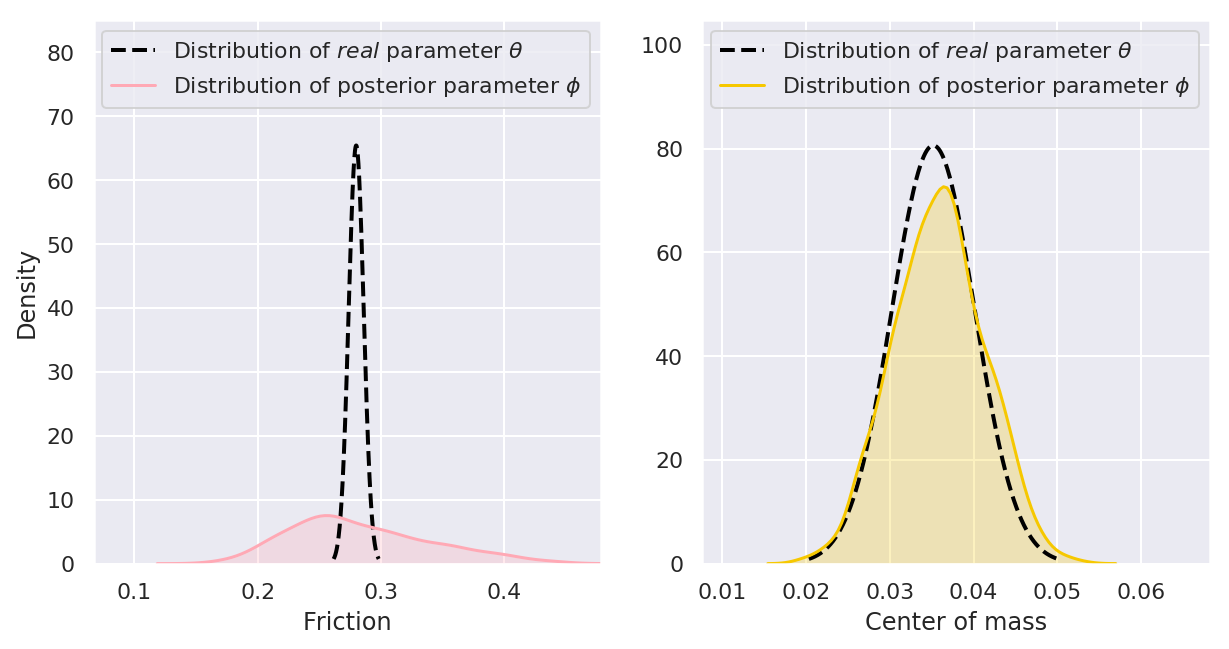
\includegraphics[width=\linewidth]{img/yumi/latent-representation/yumi_latent_encoding_3_iter}
  \caption{$\psi$ after 3rd iteration of \dettostoc{}}
\end{subfigure}
\caption{Plots show the learned parameters $\vph_{\mu, \sigma}$ of the posterior given \emph{real} samples $\vec{\xi}^{real}$ in the YuMi scenario for four iteration of \dettostoc{}.
The parameters correspond (from left-to-right) to tangential friction $\pfriction$, center of mass $\pcom$. The true distributions $\vth_{\mu, \sigma}$ are outlined in black dashes. In this scenario, \dettostoc{} struggles to match $\pfriction{}$ with the true distribution $\th_\textsc{friction}$. This is likely due to the fact that the learned policy pushes the box in small increments, and small changes in friction do not cause any noticeable difference. The posterior for all iterations can be found in the appendix.}
\label{fig:yumi_latent_space_full}
\end{figure}

\begin{figure}
    \centering
    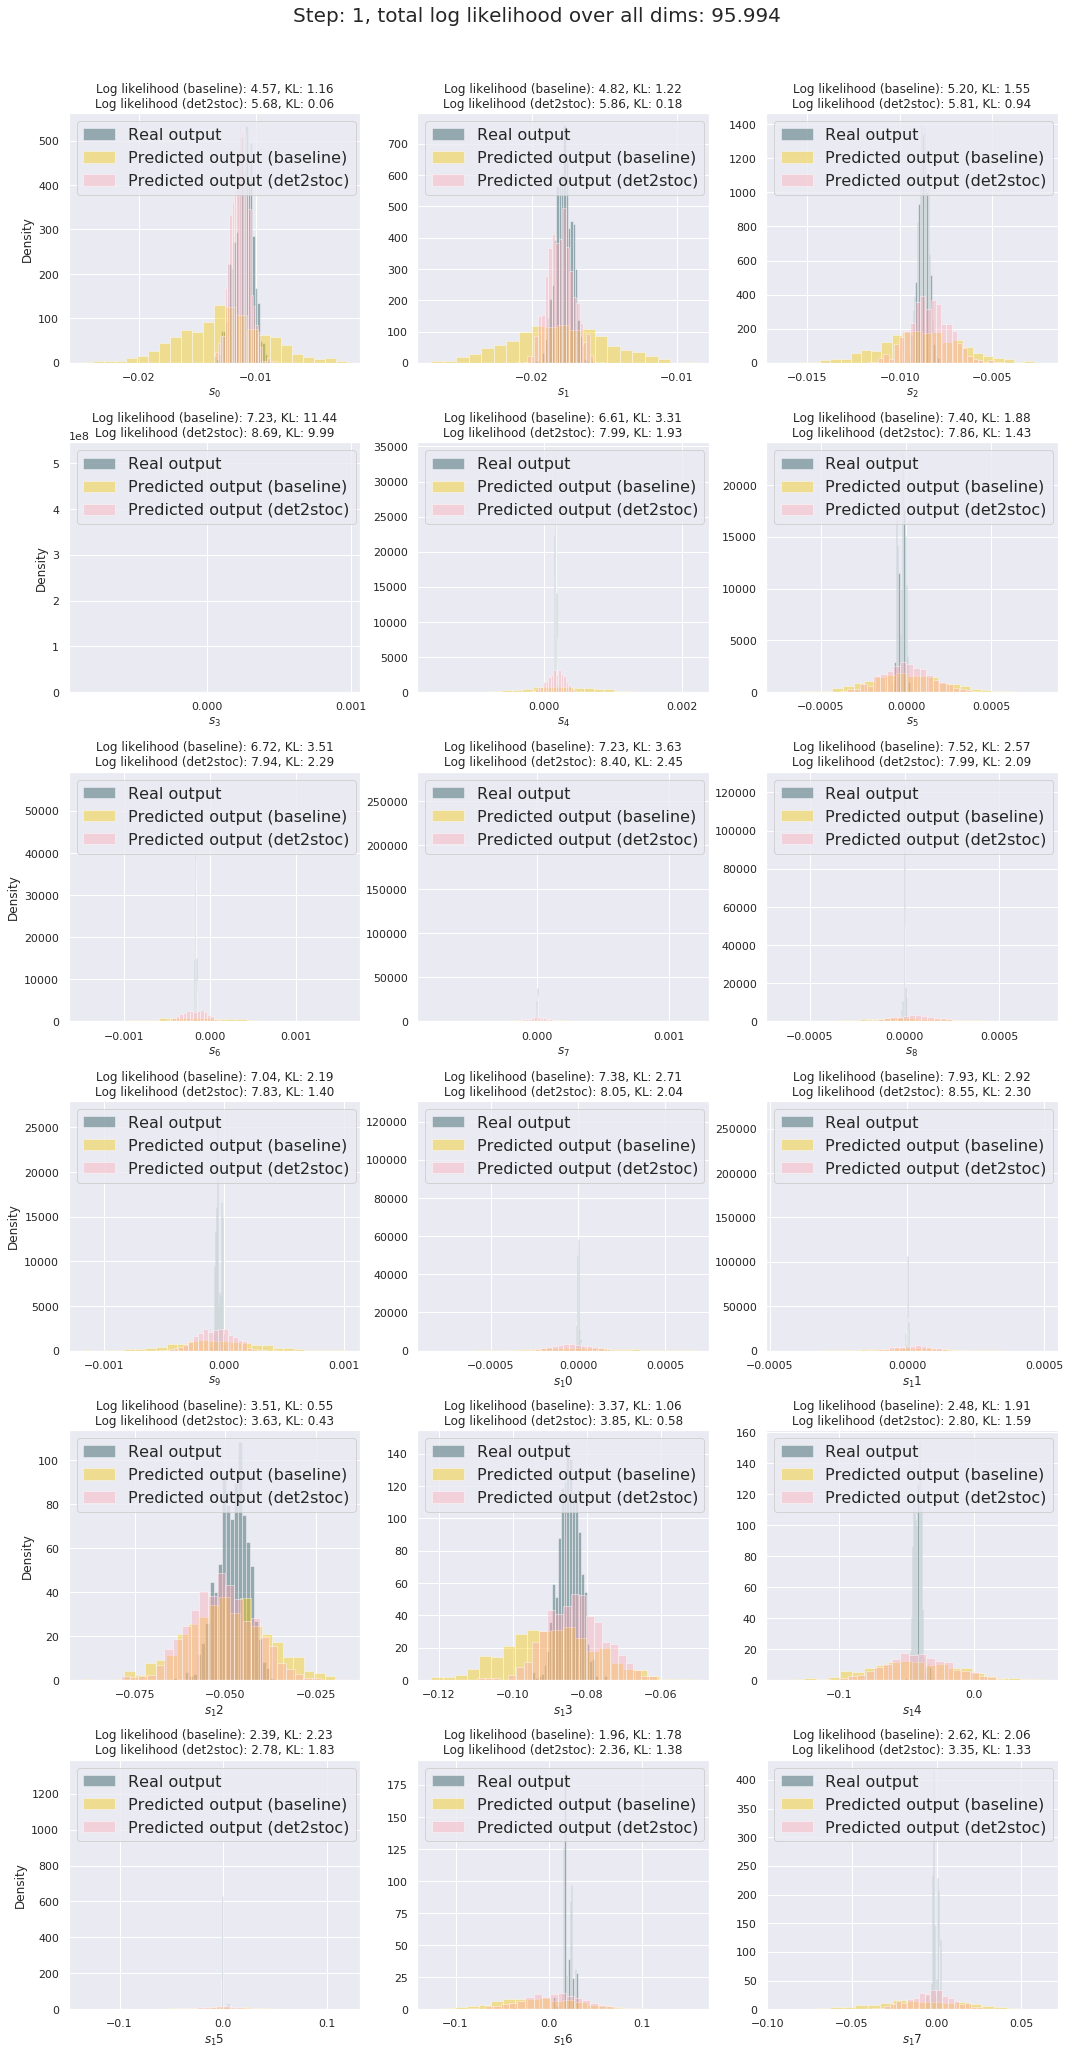
\includegraphics[width=.8\textwidth,trim=0 0 0 70,clip]{img/windyslope/output/output_distribution_step1_delta_all}
    \caption{Output predictions $\ptheta \protect\given*{\vns}{\vs}$ for a randomly sampled state at $t=1$ for iteration 4 of \dettostoc{}.}
    \label{fig:output_distribution_step1_dettostoc}
\end{figure}%
\begin{figure}
    \centering
    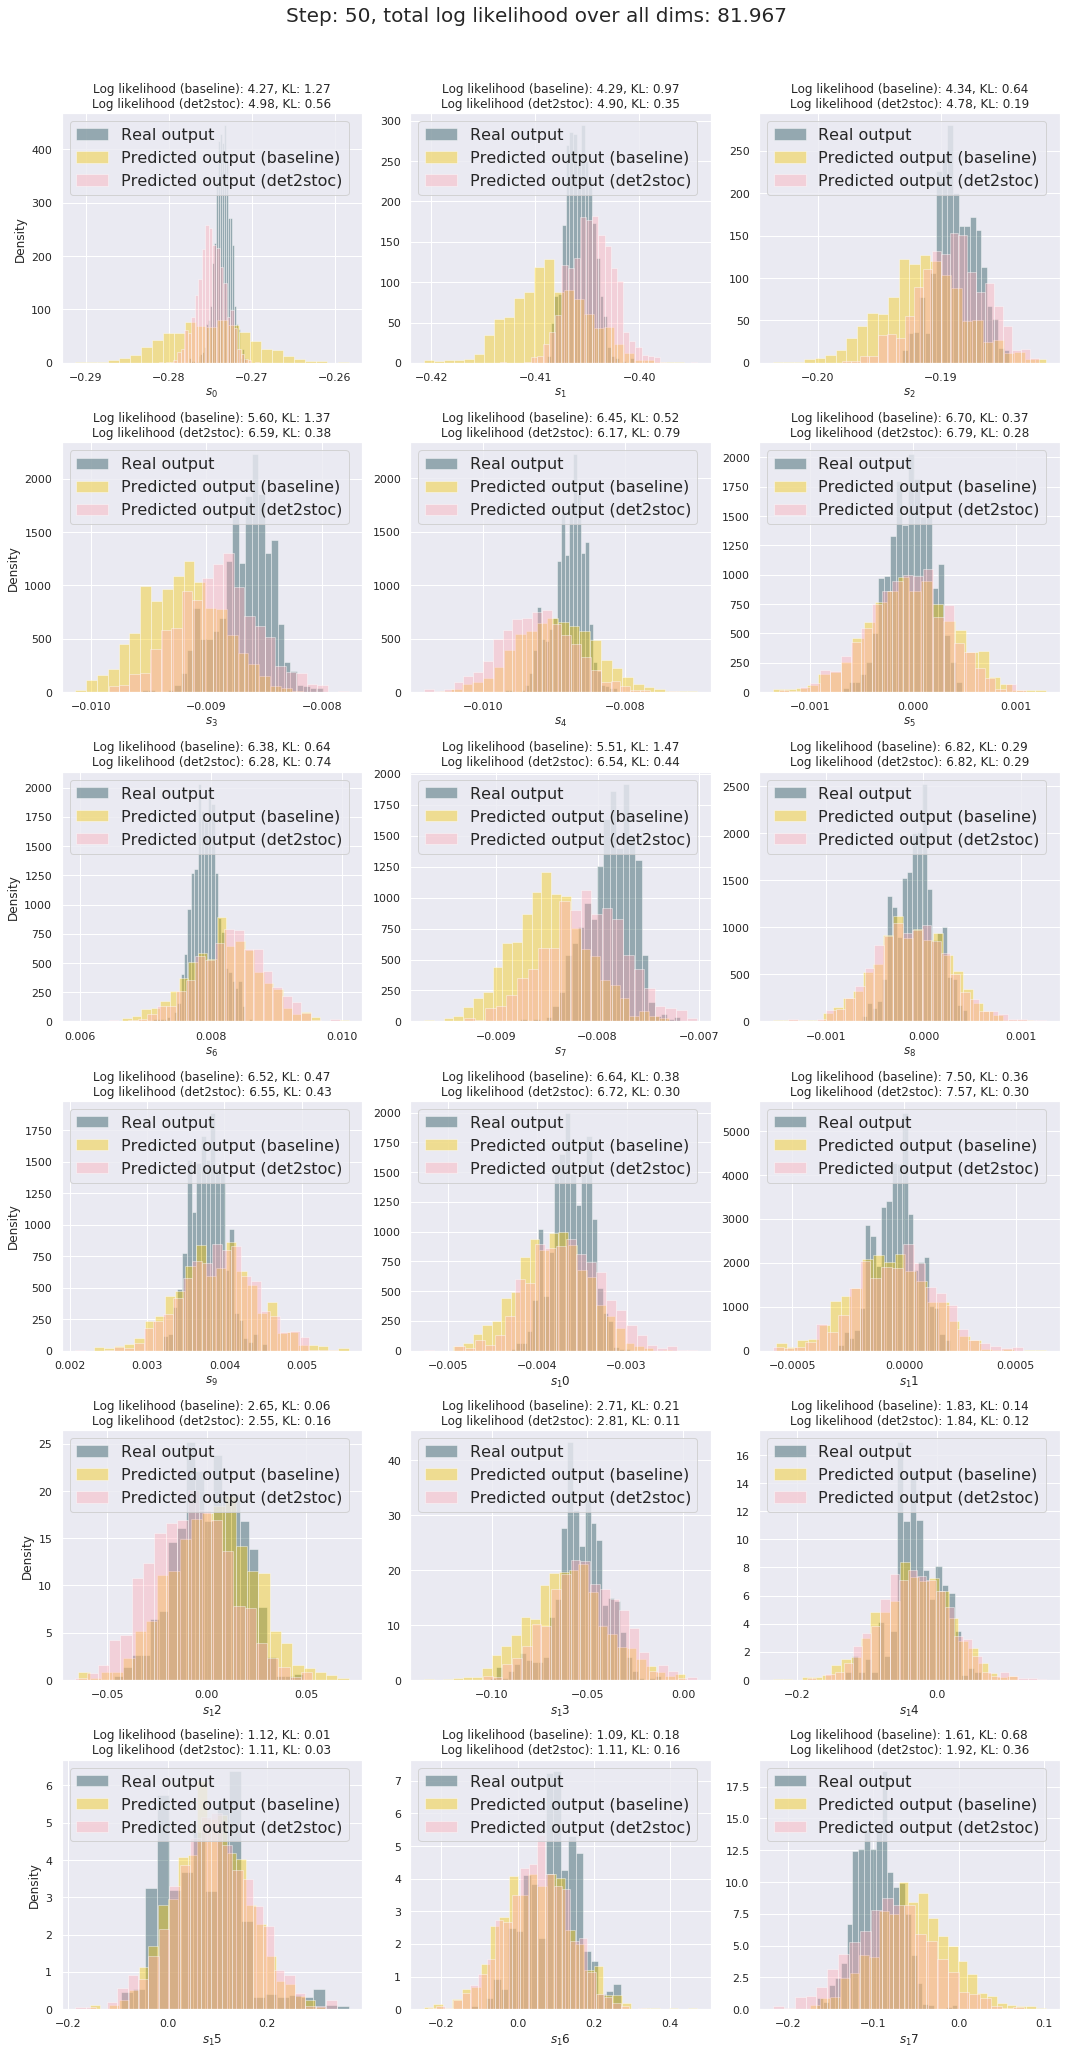
\includegraphics[width=0.8\textwidth,trim=0 0 0 70,clip]{img/windyslope/output/output_distribution_step50_delta_all}
    \caption{Output predictions $\ptheta \protect\given*{\vns}{\vs}$ for a randomly sampled state at $t=50$ for iteration 4 of \dettostoc{}.}
    \label{fig:output_distribution_step50_dettostoc}
\end{figure}
\begin{figure}
    \centering
    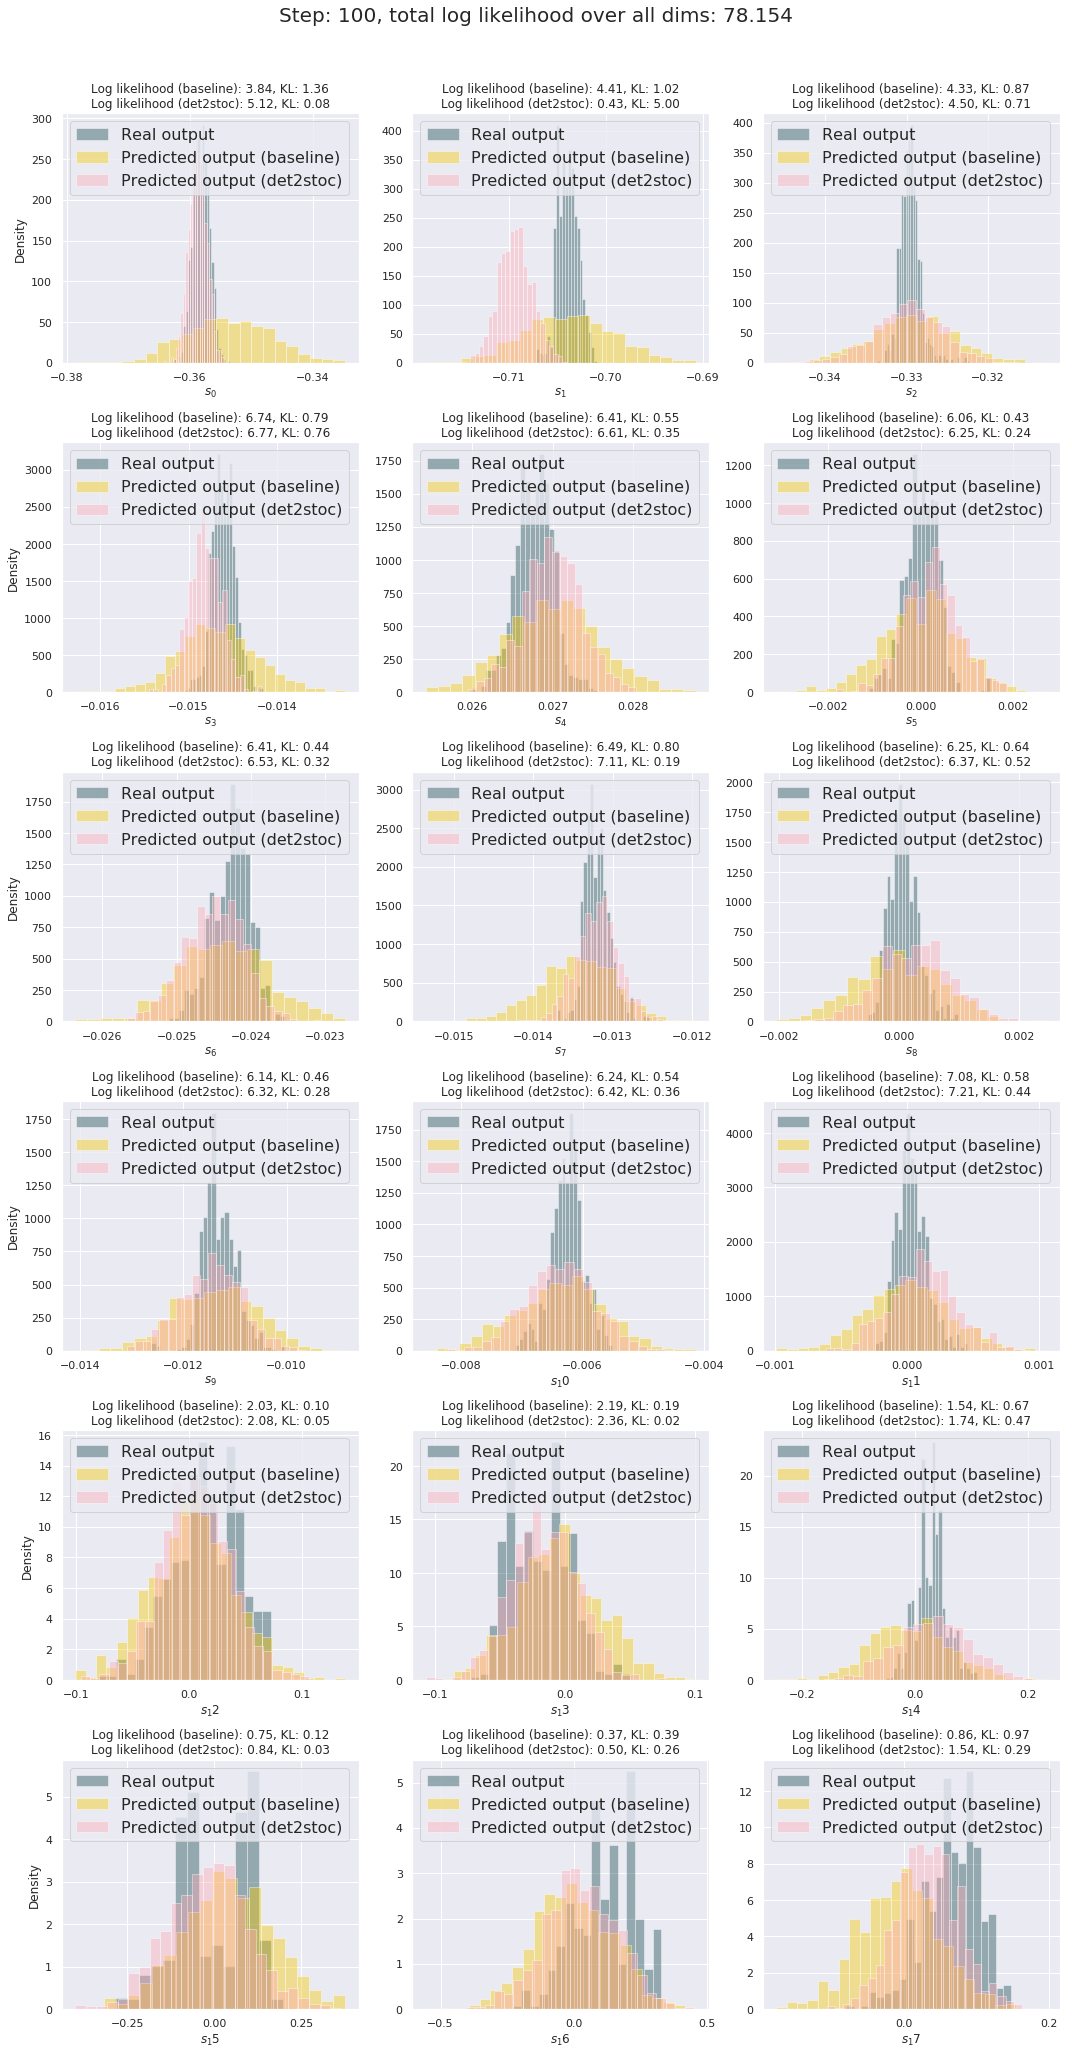
\includegraphics[width=0.8\textwidth,trim=0 0 0 70,clip]{img/windyslope/output/output_distribution_step100_delta_all}
    \caption{Output predictions $\ptheta \protect\given*{\vns}{\vs}$ for a randomly sampled state at $t=100$ for iteration 4 of \dettostoc{}.}
    \label{fig:output_distribution_step100_dettostoc}
\end{figure}


%======================================================
\tailmatter
%======================================================

\end{document}